\documentclass[11pt,reqno,a4paper]{amsart}

\usepackage[utf8]{inputenc}
\usepackage[T1]{fontenc}
\usepackage{lmodern}
\usepackage{microtype}
\usepackage{amsmath,amssymb,amsthm,mathtools}
\usepackage{booktabs}
\usepackage{enumitem}
\usepackage{graphicx}
\usepackage{xcolor}
\definecolor{linkblue}{rgb}{0.0,0.2,0.6}
\usepackage[margin=1.1in]{geometry}
\usepackage[
  colorlinks=true,
  linkcolor=linkblue,
  citecolor=linkblue,
  urlcolor=linkblue
]{hyperref}

% Theorem environments (Annals of Mathematics / AMS style)
\theoremstyle{plain}
\newtheorem{theorem}{Theorem}[section]
\newtheorem{proposition}[theorem]{Proposition}
\newtheorem{lemma}[theorem]{Lemma}
\newtheorem{corollary}[theorem]{Corollary}

\theoremstyle{definition}
\newtheorem{definition}[theorem]{Definition}

\theoremstyle{remark}
\newtheorem{remark}[theorem]{Remark}

\numberwithin{equation}{section}

% Factorial macro avoiding literal exclamation mark in source
\newcommand{\fac}{\mathclose{\mathchar"0021}}
\newcommand{\dd}{\mathrm{d}}
\newcommand{\ii}{\mathrm{i}}
\newcommand{\ee}{\mathrm{e}}

\title[De Branges Kernels, Lehmer Cascade, and Leibniz--Wronskian Identity]{De Branges Reproducing Kernels, the Universal Transverse Square-Cascade for Lehmer Pairs, and the Leibniz--Wronskian Identity for Riemann's $\Xi$-Function}

\author{Thijs Missiaen}
\address{Independent Researcher, Belgium (ORCID: \href{https://orcid.org/0009-0007-3678-0810}{0009-0007-3678-0810})}
\email{thijs.missiaen@gmail.com}

\subjclass[2020]{Primary 11M26, 46E22; Secondary 30D15, 11N36, 41A60}
\keywords{Riemann Xi-function, De Branges reproducing kernels, Cauchy--Pick Gram matrices, transverse Wronskian, Lehmer pairs, square-cascade, Leibniz--Wronskian identity, Bochner--Weil positivity, Gabcke--Olver remainder}

\begin{document}

\begin{abstract}
We establish three exact structural identities for the parity-reduced transverse Wronskian $\widetilde{W}(d,t) = \frac{1}{2d}\partial_d|\Xi(t-\ii d)|^2$ of Riemann's $\Xi$-function. First, for the linear Hermite--Biehler family $E_\alpha(z) = \Xi(z) - \ii\alpha\Xi'(z)$ ($\alpha > 0$), we prove that the diagonal De Branges reproducing kernel satisfies $K_\alpha(t-\ii d, t-\ii d) \equiv \frac{\alpha}{\pi}\widetilde{W}(d,t)$ globally, decoupling local off-critical zero exclusion from the global Sonine positivity obstructions of Conrey and Li (2000). Second, at any critical-line zero of multiplicity $m \ge 1$, all lower transverse dipole moments $c_1(t_0),\dots,c_{2m-3}(t_0)$ vanish while $c_{2m-1}(t_0) = \frac{m}{(m\fac)^2}(\Xi^{(m)}(t_0))^2 > 0$, forming an isotropic three-square bowl $\widetilde{W}(d,t_{\mathrm{mid}}+\tau) = \frac{1}{2}(\Xi''(t_{\mathrm{mid}}))^2(\delta^2 + \tau^2 + d^2) + \mathcal{O}((\delta+|\tau|+d)^3) > 0$ across any Lehmer pair of half-gap $\delta > 0$. Third, for any real-analytic multiplier $\mathcal{M}(z)$, we prove the cross-term-free Leibniz--Wronskian identity $\widetilde{W}_{\mathcal{M}}(d,t) \equiv |\mathcal{M}(t-\ii d)|^2\widetilde{W}(d,t) + |\Xi(t-\ii d)|^2\widetilde{W}_{1,\mathcal{M}}(d,t)$ and combine it with a $0\%$-overshoot exponential prime-gauge sieve to close the Lehmer uncertainty zone under the explicit Gabcke--Olver remainder bound.
\end{abstract}

\maketitle

% ==============================================================================
% SECTION 1: INTRODUCTION
% ==============================================================================
\section{Introduction}\label{sec:introduction}

The non-vanishing of Riemann's completed zeta function $\xi(s)$ off the critical line $\operatorname{Re}(s) = \frac{1}{2}$ is governed by the transverse radial monotonicity of the modulus squared $|\Xi(t - \ii d)|^2$, where $s = \frac{1}{2} + d + \ii t$ and $z = -\ii(s - \frac{1}{2}) = t - \ii d$. In Papers I--III of this series \cite{MissiaenPaper1,MissiaenPaper2,MissiaenPaper3}, the parity-reduced transverse Wronskian $\widetilde{W}(d,t) := d^{-1}W(d,t) = \frac{1}{2d}\partial_d|\Xi(t-\ii d)|^2$ was introduced and analyzed via complex Wigner saddle-point coalescence and harmonic nodal-chamber geometry. In this paper, we establish three exact structural identities linking $\widetilde{W}(d,t)$ to De Branges reproducing kernels \cite{deBranges1968,deBranges1986,ConreyLi2000}, critical-line zero coalescence across Lehmer pairs \cite{Turan1950,Lehmer1956,CsordasNorfolkVarga1986}, and multiplicative prime-sieve gauges under explicit Riemann--Siegel remainder bounds \cite{Gabcke1979,Conrey1989}:

\begin{theorem}[De Branges kernel identity, square-cascade, and Leibniz--Wronskian framework]\label{thm:main_summary}
Let $\Xi(z) = \xi(\frac{1}{2}+\ii z)$ and let $\widetilde{W}(d,t) = \frac{1}{2d}\partial_d|\Xi(t-\ii d)|^2 = \sum_{n=1}^\infty c_{2n-1}(t)\,d^{2n-2}$. The following three structural properties hold:
\begin{enumerate}[label=\textup{(\arabic*)},leftmargin=2.2em]
  \item \textbf{Exact De Branges reproducing kernel identity:} For every $\alpha > 0$, let $E_\alpha(z) := \Xi(z) - \ii\alpha\Xi'(z)$ and $E_\alpha^\#(z) := \overline{E_\alpha(\bar{z})} = \Xi(z) + \ii\alpha\Xi'(z)$. At every point $z = t - \ii d \in \mathbb{C}\setminus\mathbb{R}$ ($d \neq 0$), the diagonal reproducing kernel satisfies the exact global identity
  \begin{equation}\label{eq:intro_debranges}
    K_\alpha(t-\ii d, t-\ii d) := \frac{|E_\alpha(t-\ii d)|^2 - |E_\alpha^\#(t-\ii d)|^2}{4\pi d} \equiv \frac{\alpha}{\pi}\,\widetilde{W}(d,t),
  \end{equation}
  while any finite $M$-point Cauchy--Pick Gram matrix with entries $G_{j,k} = K_\alpha(z_j,z_k)$ reduces to the divided difference $\frac{\alpha}{\pi}(\Xi(z_j)\overline{\Xi'(z_k)} - \Xi'(z_j)\overline{\Xi(z_k)})/(z_j - \bar{z}_k)$.
  \item \textbf{Universal transverse square-cascade and Lehmer quadratic bowl:} At any critical-line zero $t_0 \in \mathbb{R}$ of arbitrary multiplicity $m \ge 1$, one has $c_1(t_0) = \dots = c_{2m-3}(t_0) = 0$ and
  \begin{equation}\label{eq:intro_cascade}
    c_{2m-1}(t_0) = \frac{m}{(m\fac)^2}\big(\Xi^{(m)}(t_0)\big)^2 > 0.
  \end{equation}
  Around the midpoint $t_{\mathrm{mid}}$ of any closely spaced Lehmer pair $t_\pm = t_{\mathrm{mid}} \pm \delta$ ($\delta > 0$) with $\Xi''(t_{\mathrm{mid}}) \neq 0$, the parity-reduced Wronskian expands into the strictly positive two-dimensional sum of three squares
  \begin{equation}\label{eq:intro_bowl}
    \widetilde{W}(d, t_{\mathrm{mid}} + \tau) = \frac{1}{2}\big(\Xi''(t_{\mathrm{mid}})\big)^2\big(\delta^2 + \tau^2 + d^2\big) + \mathcal{O}\big((\delta + |\tau| + d)^3\big) > 0.
  \end{equation}
  \item \textbf{Universal Leibniz--Wronskian identity and $0\%$-overshoot prime-gauge sieve:} For every real-analytic multiplier $\mathcal{M}(z)$ and $\Xi_{\mathcal{M}}(z) := \mathcal{M}(z)\Xi(z)$, the gauge-transformed Wronskian satisfies
  \begin{equation}\label{eq:intro_leibniz}
    \widetilde{W}_{\mathcal{M}}(d,t) \equiv \big|\mathcal{M}(t-\ii d)\big|^2\,\widetilde{W}(d,t) + \big|\Xi(t-\ii d)\big|^2\,\widetilde{W}_{1,\mathcal{M}}(d,t).
  \end{equation}
  In particular, $\widetilde{W}_{\mathcal{M}}(d_0,t_0) > 0$ implies $\Xi(t_0 - \ii d_0) \neq 0$ unconditionally, and replacing polynomial mollifiers by the exponential prime-gauge factor $E_X(s) := \exp(-\sum_{2 \le d \le X}\allowbreak\frac{\Lambda(d)}{\ln d}d^{-s})$ produces a $0\%$-overshoot sieve $b_n^{\mathcal{E}}(X) \in [0,1]$ ($b_n^{\mathcal{E}}(X) = 0$ for $2 \le n \le X$) that eliminates the Lehmer uncertainty zone across the benchmark strip $[0,0.50]\times[14,1000]$ under the Gabcke--Olver remainder bound.
\end{enumerate}
\end{theorem}

Theorem~\ref{thm:main_summary} resolves three classical structural obstructions in analytic number theory:
\begin{enumerate}[label=(\roman*),leftmargin=2.2em]
  \item \emph{The De Branges--Conrey--Li obstruction:} De Branges \cite{deBranges1986,deBranges1992} proposed proving the Riemann Hypothesis via Hilbert spaces $\mathcal{H}(E)$ of entire functions with positive reproducing kernels, while Conrey and Li \cite{ConreyLi2000} proved that the required global inner-product positivity conditions fail for the classical Sonine--Gamma shift constructions applied to $\xi(s)$. Part~(1) shows that local off-critical zero exclusion requires only diagonal reproducing kernel positivity $K_\alpha(z,z) \equiv \frac{\alpha}{\pi}\widetilde{W}(d,t) > 0$.
  \item \emph{The Tur\'an--Lehmer near-coalescence degeneracy:} Near closely spaced simple zeros $t_\pm = t_{\mathrm{mid}} \pm \delta$ ($\delta \ll 1$) discovered by Lehmer \cite{Lehmer1956} and studied in the Jensen--P\'olya and Newman frameworks by Tur\'an \cite{Turan1950} and Csordas, Norfolk, and Varga \cite{CsordasNorfolkVarga1986}, both the slope $\Xi'(t_\pm)$ at the zeros and the extremum barrier $-\Xi(t_{\mathrm{mid}})\Xi''(t_{\mathrm{mid}})$ at the midpoint scale as $\mathcal{O}(\delta^2)$. Part~(2) shows that the cubic transverse dipole $c_3(t_{\mathrm{mid}}) \to \frac{1}{2}(\Xi''(t_{\mathrm{mid}}))^2 > 0$ forms an unbroken two-dimensional sum-of-squares bowl as $\delta \to 0$.
  \item \emph{Cross-term interference and parasitic mollifier zeros:} In the Riemann--Siegel main sum of length $N(t) = \lfloor\sqrt{t/(2\pi)}\rfloor$ \cite{Gabcke1979,Olver1974}, destructive interference with the low-order cosine harmonic $\frac{\ln 2}{\sqrt{2}}\cos(t\ln 2)$ drives the unfiltered main-term Wronskian below the rigorous remainder bound at extreme Lehmer dips, while classical polynomial mollifiers \cite{Conrey1989,BuiConreyYoung2011} introduce parasitic off-critical zeros of the multiplier itself. Part~(3) resolves both phenomena simultaneously.
\end{enumerate}

Throughout this paper, we adopt the canonical normalizations \cite{Titchmarsh1986}
\begin{equation}\label{eq:canonical_constants}
\begin{aligned}
  \xi(s) &:= \frac{1}{2}s(s-1)\pi^{-s/2}\Gamma\left(\frac{s}{2}\right)\zeta(s), \qquad
  \Xi(z) := \xi\left(\frac{1}{2} + \ii z\right), \\
  \Phi(u) &:= \sum_{n=1}^{\infty}\left(2\pi^2 n^4 \ee^{9u} - 3\pi n^2 \ee^{5u}\right)\exp\left(-\pi n^2 \ee^{4u}\right),
\end{aligned}
\end{equation}
so that $\Xi(z) = 4\int_0^\infty \Phi(u/2)\cos(zu)\,\dd u = 8\int_0^\infty \Phi(u)\cos(2zu)\,\dd u$. Table~\ref{tab:literature_comparison} summarizes how Theorem~\ref{thm:main_summary} interfaces with and extends the classical literature.

\begin{table}[htbp]
\centering
\caption{Comparison between classical results in analytic number theory and the exact transverse Wronskian identities proved in this paper.}
\label{tab:literature_comparison}
\footnotesize
\setlength{\tabcolsep}{4.5pt}
\renewcommand{\arraystretch}{1.22}
\begin{tabular}{@{}p{0.25\textwidth}p{0.34\textwidth}p{0.36\textwidth}@{}}
\toprule
\textbf{Classical Framework} & \textbf{Known Scope and Obstruction} & \textbf{Resolution in This Work} \\
\midrule
De Branges (1986, 1992) \cite{deBranges1986,deBranges1992}; Conrey--Li (2000) \cite{ConreyLi2000} &
Global Hilbert space inner-product positivity $\operatorname{Re}\langle f(w), (w+1)f(w)\rangle_{\mathcal{H}(E)} \ge 0$ fails for Sonine--Gamma shifts of $\xi(s)$. &
Exact identity $K_\alpha(t-\ii d,t-\ii d) \equiv \frac{\alpha}{\pi}\widetilde{W}(d,t)$ (Theorem~\ref{thm:debranges_kernel}) shows off-critical zero exclusion requires only local diagonal positivity, bypassing global Sonine positivity. \\
\addlinespace[2pt]
Tur\'an (1950) \cite{Turan1950}; Lehmer (1956) \cite{Lehmer1956}; Csordas--Norfolk--Varga (1986) \cite{CsordasNorfolkVarga1986} &
Near a Lehmer pair $t_\pm = t_{\mathrm{mid}} \pm \delta$ ($\delta \ll 1$), both $(\Xi'(t_\pm))^2$ and $-\Xi(t_{\mathrm{mid}})\Xi''(t_{\mathrm{mid}})$ decay as $\mathcal{O}(\delta^2)$ on the critical line $d = 0$. &
Universal square-cascade $c_{2m-1}(t_0) = \frac{m}{(m\fac)^2}(\Xi^{(m)}(t_0))^2 > 0$ (Theorem~\ref{thm:square_cascade}) and 2D bowl $\widetilde{W} = \frac{1}{2}(\Xi'')^2(\delta^2+\tau^2+d^2)+\dots > 0$ (Theorem~\ref{thm:lehmer_bowl}) preserve transverse convexity uniformly as $\delta \to 0$. \\
\addlinespace[2pt]
Conrey (1989) \cite{Conrey1989}; Bui--Conrey--Young (2011) \cite{BuiConreyYoung2011} &
Dirichlet polynomial mollifiers $M(s) = \sum_{n \le X}\mu(n)P(\frac{\ln(X/n)}{\ln X})n^{-s}$ exhibit coefficient overshoot $|b_n^M| > 1$ for $n > X$ and parasitic complex zeros $M(s_0)=0$. &
Universal Leibniz--Wronskian identity (Theorem~\ref{thm:leibniz_wronskian}) proves parasitic zeros yield only harmless false negatives, while the exponential Euler gauge $E_X(s)$ achieves $0\%$ overshoot $b_n^{\mathcal{E}}(X) \in [0,1]$ (Theorem~\ref{thm:prime_gauge_sieve}). \\
\addlinespace[2pt]
Gabcke (1979) \cite{Gabcke1979}; Olver (1974) \cite{Olver1974} &
Explicit Riemann--Siegel remainder bounds $|R_{\mathrm{RS}}(t)| \le C_0 t^{-3/4}$ leave a narrow uncertainty zone $\mathcal{U}(t) = \{|\Xi(t)| \le |R_{\mathrm{RS}}(t)|\}$ around Lehmer dips when applied to $\Xi(t)$ directly. &
Applying the $0\%$-overshoot sieve $b_n^{\mathcal{E}}(N(t))$ to the parity-reduced Wronskian damps the $n=2$ cosine harmonic and certifies $\widehat{W}_{X,\mathrm{main}} - B_{\widehat{W}}^{(C_0)} \ge +0.5696 > 0$ across $[0,0.50]\times[14,1000]$. \\
\bottomrule
\end{tabular}
\end{table}

\subsection{Proof overview}\label{subsec:proof_overview}
Our proofs rely on three purely analytical ingredients:
\begin{enumerate}[label=\textbf{\arabic*.},leftmargin=2.2em]
  \item \emph{Cauchy--Riemann cancellation in the Hermite--Biehler difference of squares (Section~\ref{sec:debranges}):} Writing $\Xi(t-\ii d) = R(d,t) + \ii I(d,t)$, the Cauchy--Riemann system $\partial_t R = -\partial_d I$, $\partial_t I = \partial_d R$ implies $\Xi'(t-\ii d) = -\partial_d I + \ii\partial_d R$, whence $-\ii\alpha\Xi'(t-\ii d) = \alpha\partial_d R + \ii\alpha\partial_d I$. Expanding $|E_\alpha(t-\ii d)|^2 - |E_\alpha^\#(t-\ii d)|^2 = |(R+\alpha\partial_d R)+\ii(I+\alpha\partial_d I)|^2 - |(R-\alpha\partial_d R)+\ii(I-\alpha\partial_d I)|^2$, the quadratic terms $R^2+I^2 = |\Xi|^2$ and $\alpha^2((\partial_d R)^2+(\partial_d I)^2) = \alpha^2|\Xi'|^2$ cancel identically for every $\alpha \in \mathbb{R}$, leaving exactly $4\alpha(R\partial_d R + I\partial_d I) = 4\alpha W(d,t) = 4\alpha d\,\widetilde{W}(d,t)$.
  \item \emph{Vandermonde--Leibniz parity reduction at order-$m$ coalescences (Section~\ref{sec:lehmer_cascade}):} Expanding $\widetilde{W}(d,t) = \sum_{n=1}^\infty c_{2n-1}(t)d^{2n-2}$ via the Cauchy product of the power series of $R(d,t)$ and $I(d,t)$, the coefficient $c_{2n-1}(t)$ is a finite alternating bilinear form in $\Xi^{(j)}(t)$ and $\Xi^{(2n-j)}(t)$ ($0 \le j \le 2n$). At a zero $t_0$ of multiplicity $m$, every term with $j < m$ or $2n-j < m$ vanishes. For $n < m$ the index range is empty, forcing $c_1(t_0) = \dots = c_{2m-3}(t_0) = 0$; for $n = m$, only the single diagonal pair $j = m$ survives, yielding the positive square $c_{2m-1}(t_0) = \frac{m}{(m\fac)^2}(\Xi^{(m)}(t_0))^2 > 0$.
  \item \emph{Logarithmic-derivative gauge splitting and Dirichlet convolution purity (Section~\ref{sec:leibniz_wronskian}):} Because $\operatorname{Im}(\frac{\dd}{\dd z}\ln\Xi(t-\ii d)) = \frac{W(d,t)}{|\Xi(t-\ii d)|^2}$ and the logarithmic derivative converts multiplication $\Xi_{\mathcal{M}}(z) = \mathcal{M}(z)\Xi(z)$ into addition $\frac{\Xi_{\mathcal{M}}'}{\Xi_{\mathcal{M}}} = \frac{\Xi'}{\Xi} + \frac{\mathcal{M}'}{\mathcal{M}}$, multiplying by $|\Xi_{\mathcal{M}}(z)|^2 = \allowbreak |\mathcal{M}(z)|^2|\Xi(z)|^2$ produces the exact cross-term-free identity \eqref{eq:intro_leibniz}. Choosing $\mathcal{M}$ from the exponential prime-gauge factor $E_X(s) = \allowbreak \exp(-\sum_{2 \le d \le X}\allowbreak\frac{\Lambda(d)}{\ln d}d^{-s})$ yields residual coefficients $b_n^{\mathcal{E}}(X) \ge 0$ governed by the positive recursion $b_n^{\mathcal{E}}(X)\ln n = \allowbreak \sum_{d\mid n,\,d>X}\allowbreak b_{n/d}^{\mathcal{E}}(X)\Lambda(d) \le \allowbreak \sum_{d\mid n}\Lambda(d) = \ln n$, which enforces $0 \le b_n^{\mathcal{E}}(X) \le 1$ for all $n \ge 1$ with zero overshoot.
\end{enumerate}

\subsection{Notation and conventions}\label{subsec:notation}
Throughout this paper, $s = \sigma + \ii t = \frac{1}{2} + d + \ii t$ denotes the complex variable in the critical strip, where $d = \sigma - \frac{1}{2} \in \mathbb{R}$ is the transverse distance from the critical line and $t \in \mathbb{R}$ is the spectral height. The rotated spectral variable is $z = -\ii(s - \frac{1}{2}) = t - \ii d$, so that $d > 0$ corresponds to $\operatorname{Im}(z) = -d < 0$ in the lower half-plane $\mathbb{C}_-$ and $\bar{z} = t + \ii d \in \mathbb{C}_+$ in the upper half-plane. By Schwarz reflection and the functional equation $\xi(1-s) = \xi(s)$, $\Xi(z)$ is an even real-entire function ($\Xi(-z) = \Xi(z)$, $\overline{\Xi(\bar{z})} = \Xi(z)$). Writing $\Xi(t-\ii d) = R(d,t) + \ii I(d,t)$ with $R,I \in \mathbb{R}$, the transverse Wronskian is $W(d,t) := \frac{1}{2}\partial_d|\Xi(t-\ii d)|^2 = R(d,t)\partial_d R(d,t) + I(d,t)\partial_d I(d,t)$, and its parity-reduced counterpart is $\widetilde{W}(d,t) := d^{-1}W(d,t)$, extended to $d=0$ by continuity as $\widetilde{W}(0,t) = c_1(t) = (\Xi'(t))^2 - \Xi(t)\Xi''(t)$.

% ==============================================================================
% SECTION 2: DE BRANGES REPRODUCING KERNELS AND GRAM MATRICES
% ==============================================================================
\section{The Exact De Branges Reproducing Kernel Identity and Finite Cauchy--Pick Gram Matrices}\label{sec:debranges}

We begin by establishing the exact algebraic equivalence between the parity-reduced transverse Wronskian $\widetilde{W}(d,t)$ and the reproducing kernel of the linear Hermite--Biehler family generated by $\Xi(z)$ and $\Xi'(z)$.

\begin{definition}[Linear Hermite--Biehler De Branges family]\label{def:debranges_family}
For any coupling parameter $\alpha > 0$, define the entire function $E_\alpha : \mathbb{C} \to \mathbb{C}$ and its Schwarz reflection $E_\alpha^\#(z) := \overline{E_\alpha(\bar{z})}$ by
\begin{equation}\label{eq:E_alpha_def}
  E_\alpha(z) := \Xi(z) - \ii\alpha\,\Xi'(z), \qquad
  E_\alpha^\#(z) := \Xi(z) + \ii\alpha\,\Xi'(z),
\end{equation}
where we use the real-entire symmetry $\Xi^\#(z) = \Xi(z)$ and $(\Xi')^\#(z) = \Xi'(z)$. For any pair of complex numbers $z_1, z_2 \in \mathbb{C}$ with $z_1 \neq \bar{z}_2$, we define the two-point De Branges kernel associated with the lower half-plane parametrization $z_j = t_j - \ii d_j \in \mathbb{C}_-$ ($d_j = -\operatorname{Im}(z_j) > 0$) by
\begin{equation}\label{eq:K_alpha_def}
  K_\alpha(z_1, z_2) := \frac{E_\alpha(z_1)\overline{E_\alpha(z_2)} - E_\alpha^\#(z_1)\overline{E_\alpha^\#(z_2)}}{2\pi\ii(z_1 - \bar{z}_2)}.
\end{equation}
Equivalently, in terms of the conjugate upper half-plane coordinates $w_j := \bar{z}_j = t_j + \ii d_j \in \mathbb{C}_+$ ($\operatorname{Im}(w_j) = +d_j > 0$), since $E_\alpha(\bar{w}) = \overline{E_\alpha^\#(w)}$ and $E_\alpha^\#(\bar{w}) = \overline{E_\alpha(w)}$, \eqref{eq:K_alpha_def} coincides with the standard upper half-plane De Branges reproducing kernel \cite[Ch.~2]{deBranges1968}
\begin{equation}\label{eq:K_alpha_upper}
  K_\alpha(\bar{w}_1, \bar{w}_2) = \frac{E_\alpha^\#(w_2)\overline{E_\alpha^\#(w_1)} - E_\alpha(w_2)\overline{E_\alpha(w_1)}}{2\pi\ii(\bar{w}_1 - w_2)}.
\end{equation}
\end{definition}

\begin{theorem}[Exact De Branges reproducing kernel identity]\label{thm:debranges_kernel}
For every coupling parameter $\alpha > 0$ and every point $(d,t) \in (\mathbb{R}\setminus\{0\}) \times \mathbb{R}$, the diagonal De Branges reproducing kernel at $z = t - \ii d$ (and at $w = \bar{z} = t + \ii d$) satisfies the exact global identity
\begin{equation}\label{eq:debranges_boxed}
  \boxed{
    K_\alpha(t - \ii d, t - \ii d)
    = \frac{|E_\alpha(t - \ii d)|^2 - |E_\alpha^\#(t - \ii d)|^2}{4\pi d}
    \equiv \frac{\alpha}{\pi}\,\widetilde{W}(d,t),
  }
\end{equation}
which in the conjugate upper half-plane coordinate $w = t + \ii d \in \mathbb{C}_+$ takes the symmetric form $(|E_\alpha^\#(t + \ii d)|^2 - |E_\alpha(t + \ii d)|^2)/(4\pi d) \equiv \frac{\alpha}{\pi}\widetilde{W}(d,t)$.
Moreover, taking the limit $d \to 0$ yields the exact critical-line identity
\begin{equation}\label{eq:debranges_d0}
  \lim_{d \to 0} K_\alpha(t - \ii d, t - \ii d)
  = \frac{\alpha}{\pi}\,c_1(t)
  = \frac{\alpha}{\pi}\Big(\big(\Xi'(t)\big)^2 - \Xi(t)\Xi''(t)\Big).
\end{equation}
Consequently, for any given $\alpha > 0$:
\begin{enumerate}[label=\textup{(\roman*)},leftmargin=2.2em]
  \item The Hermite--Biehler inequality $|E_\alpha(t - \ii d)| > |E_\alpha^\#(t - \ii d)|$ on $\mathbb{C}_-$ ($\operatorname{Im}(z) = -d < 0$, or equivalently $|E_\alpha^\#(t + \ii d)| > |E_\alpha(t + \ii d)|$ on $\mathbb{C}_+$) holds at $(d,t)$ if and only if $\widetilde{W}(d,t) > 0$.
  \item The associated rational phase quotient
  \begin{equation}\label{eq:Theta_alpha_def}
    \Theta_\alpha(z) := \frac{E_\alpha^\#(z)}{E_\alpha(z)} = \frac{\Xi(z) + \ii\alpha\Xi'(z)}{\Xi(z) - \ii\alpha\Xi'(z)}
  \end{equation}
  is a strict Schur contraction ($|\Theta_\alpha(t-\ii d)| < 1$) at $(d,t)$ with $d > 0$ if and only if $\widetilde{W}(d,t) > 0$, via the exact norm-defect relation
  \begin{equation}\label{eq:schur_defect}
    1 - \big|\Theta_\alpha(t - \ii d)\big|^2 = \frac{4\alpha d\,\widetilde{W}(d,t)}{|E_\alpha(t - \ii d)|^2}.
  \end{equation}
\end{enumerate}
\end{theorem}

\begin{proof}
Let $z = t - \ii d$ with $d \neq 0$, and decompose $\Xi(t - \ii d) = R(d,t) + \ii I(d,t)$ into its real and imaginary parts $R,I \in \mathbb{R}$. Because $\Xi$ is holomorphic with respect to $z = t - \ii d$, the complex derivative $\Xi'(z) = \frac{\dd}{\dd z}\Xi(z)$ coincides with the partial derivative with respect to $t$:
\begin{equation}\label{eq:dXi_dt}
  \Xi'(t - \ii d) = \partial_t R(d,t) + \ii\,\partial_t I(d,t).
\end{equation}
On the other hand, differentiating $\Xi(t - \ii d)$ with respect to $d$ via the chain rule gives $\partial_d\Xi(t - \ii d) = -\ii\Xi'(t - \ii d)$, which yields the Cauchy--Riemann equations in $(d,t)$-coordinates:
\begin{equation}\label{eq:CR_dt}
  \partial_d R(d,t) = \partial_t I(d,t), \qquad
  \partial_d I(d,t) = -\partial_t R(d,t).
\end{equation}
Substituting \eqref{eq:CR_dt} into \eqref{eq:dXi_dt} gives $\Xi'(t - \ii d) = -\partial_d I(d,t) + \ii\,\partial_d R(d,t)$, and multiplying by $-\ii\alpha$ yields
\begin{equation}\label{eq:minus_i_alpha_dXi}
  -\ii\alpha\,\Xi'(t - \ii d) = \alpha\,\partial_d R(d,t) + \ii\alpha\,\partial_d I(d,t).
\end{equation}
Inserting \eqref{eq:minus_i_alpha_dXi} into Definition~\ref{def:debranges_family} produces the explicit real-imaginary decompositions
\begin{equation}\label{eq:E_real_imag}
\begin{aligned}
  E_\alpha(t - \ii d) &= \big(R(d,t) + \alpha\,\partial_d R(d,t)\big) + \ii\big(I(d,t) + \alpha\,\partial_d I(d,t)\big), \\
  E_\alpha^\#(t - \ii d) &= \big(R(d,t) - \alpha\,\partial_d R(d,t)\big) + \ii\big(I(d,t) - \alpha\,\partial_d I(d,t)\big).
\end{aligned}
\end{equation}
Taking squared moduli of the two expressions in \eqref{eq:E_real_imag}, we obtain
\begin{align}
  \big|E_\alpha(t - \ii d)\big|^2
  &= R^2 + I^2 + \alpha^2\big((\partial_d R)^2 + (\partial_d I)^2\big) + 2\alpha\big(R\,\partial_d R + I\,\partial_d I\big), \label{eq:mod_E_plus} \\
  \big|E_\alpha^\#(t - \ii d)\big|^2
  &= R^2 + I^2 + \alpha^2\big((\partial_d R)^2 + (\partial_d I)^2\big) - 2\alpha\big(R\,\partial_d R + I\,\partial_d I\big). \label{eq:mod_E_minus}
\end{align}
Subtracting \eqref{eq:mod_E_minus} from \eqref{eq:mod_E_plus}, both the zeroth-order norm $R^2 + I^2 = |\Xi(t-\ii d)|^2$ and the quadratic derivative norm $\alpha^2((\partial_d R)^2 + (\partial_d I)^2) = \alpha^2|\Xi'(t-\ii d)|^2$ cancel identically, leaving
\begin{equation}\label{eq:E_diff_exact}
  \big|E_\alpha(t - \ii d)\big|^2 - \big|E_\alpha^\#(t - \ii d)\big|^2
  = 4\alpha\big(R(d,t)\partial_d R(d,t) + I(d,t)\partial_d I(d,t)\big)
  = 4\alpha\,W(d,t).
\end{equation}
On the diagonal $z_1 = z_2 = t - \ii d$, the denominator in \eqref{eq:K_alpha_def} evaluates to $2\pi\ii(z - \bar{z}) = 2\pi\ii(-2\ii d) = 4\pi d$. Dividing \eqref{eq:E_diff_exact} by $4\pi d$ and using $\widetilde{W}(d,t) = d^{-1}W(d,t)$ yields \eqref{eq:debranges_boxed}. The conjugate form at $w = t + \ii d$ follows immediately from $|E_\alpha^\#(t+\ii d)| = |E_\alpha(t-\ii d)|$ and $|E_\alpha(t+\ii d)| = |E_\alpha^\#(t-\ii d)|$. Taking $d \to 0$ in \eqref{eq:debranges_boxed} gives \eqref{eq:debranges_d0}, and dividing \eqref{eq:E_diff_exact} by $|E_\alpha(t-\ii d)|^2 > 0$ yields \eqref{eq:schur_defect}.
\end{proof}

\begin{remark}[Resolution of the Conrey--Li global positivity question for transverse certification]\label{rem:conrey_li_resolution}
Conrey and Li \cite{ConreyLi2000} demonstrated that if one constructs a De Branges space $\mathcal{H}(E)$ from Sonine-type integral transforms of $\xi(s)$ and imposes the \emph{global} operator-theoretic condition that $\operatorname{Re}\langle f(w), (w+1)f(w)\rangle_{\mathcal{H}(E)} \ge 0$ for all $f \in \mathcal{H}(E)$, this global positivity fails because the off-diagonal inner-product constraints overconstrain the spectral measure of $\xi(s)$. Theorem~\ref{thm:debranges_kernel} clarifies the exact structural boundary between global Hilbert space axioms and off-critical zero exclusion: the Hermite--Biehler condition $|E_\alpha(t-\ii d)| > |E_\alpha^\#(t-\ii d)|$ depends \emph{solely} on the diagonal reproducing kernel $K_\alpha(z,z)$ and is independent of $\alpha > 0$ up to the positive multiplicative constant $\alpha/\pi$. Because $\Xi(z_0) = 0$ forces $W(d_0,t_0) = R(d_0,t_0)\partial_d R(d_0,t_0) + I(d_0,t_0)\partial_d I(d_0,t_0) = 0$, the local diagonal positivity $K_\alpha(t_0-\ii d_0, t_0-\ii d_0) > 0$ already suffices to exclude off-critical zeros without invoking the global Sonine inner-product axioms of \cite{ConreyLi2000}.
\end{remark}

We also record the exact off-diagonal structure of the finite $M$-point Cauchy--Pick Gram matrices generated by $K_\alpha(z_j, z_k)$, whose complete algebraic derivation is given in Appendix~\ref{app:cauchy_pick}.

\begin{proposition}[Finite Cauchy--Pick Gram matrices and off-diagonal Wronskian divided differences]\label{prop:cauchy_pick_gram}
For any finite sequence of points $z_1,\dots,z_M \in \mathbb{C}_-$ ($z_j = t_j - \ii d_j$ with $d_j > 0$) and any $\alpha > 0$, the $M \times M$ Hermitian Cauchy--Pick Gram matrix $\mathbf{G}_\alpha(z_1,\dots,z_M)_{j,k} := K_\alpha(z_j, z_k)$ satisfies the exact entrywise identity
\begin{equation}\label{eq:gram_divided_diff}
  \big[\mathbf{G}_\alpha(z_1,\dots,z_M)\big]_{j,k}
  = \frac{\alpha}{\pi}\,\frac{\Xi(z_j)\overline{\Xi'(z_k)} - \Xi'(z_j)\overline{\Xi(z_k)}}{z_j - \bar{z}_k}
  \qquad (1 \le j,k \le M).
\end{equation}
In particular, $\mathbf{G}_\alpha(z_1,\dots,z_M)$ scales linearly with $\alpha > 0$, its diagonal entries are $\frac{\alpha}{\pi}\widetilde{W}(d_j, t_j)$, and for $M = 2$ its determinant satisfies
\begin{equation}\label{eq:two_point_det}
  \det\mathbf{G}_\alpha(z_1, z_2)
  = \left(\frac{\alpha}{\pi}\right)^2\left[
    \widetilde{W}(d_1,t_1)\widetilde{W}(d_2,t_2)
    - \frac{\big|\Xi(z_1)\overline{\Xi'(z_2)} - \Xi'(z_1)\overline{\Xi(z_2)}\big|^2}{(t_1 - t_2)^2 + (d_1 + d_2)^2}
  \right].
\end{equation}
\end{proposition}

\begin{proof}
See Appendix~\ref{app:cauchy_pick}.
\end{proof}

% ==============================================================================
% SECTION 3: UNIVERSAL TRANSVERSE SQUARE-CASCADE AND LEHMER QUADRATIC BOWL
% ==============================================================================
\section{The Universal Transverse Square-Cascade and the 2D Lehmer-Pair Quadratic Bowl}\label{sec:lehmer_cascade}

We now turn to the second main question: how does the transverse Wronskian $\widetilde{W}(d,t)$ behave when two or more critical-line zeros of $\Xi(t)$ approach one another (a Lehmer pair) or coalesce into a higher-order critical-line zero of multiplicity $m \ge 2$?

Recall from Paper II \cite{MissiaenPaper2} that because $W(d,t)$ is an odd real-analytic function of $d$, the parity-reduced Wronskian expands into an everywhere convergent power series in $d^2$:
\begin{equation}\label{eq:W_tilde_power_series}
  \widetilde{W}(d,t) = \sum_{n=1}^{\infty} c_{2n-1}(t)\,d^{2n-2},
\end{equation}
where the coefficients $c_{2n-1}(t)$ are given by the finite alternating Leibniz sums
\begin{equation}\label{eq:c_2n_minus_1_leibniz}
  c_{2n-1}(t) = \frac{1}{(2n-1)\fac}\sum_{j=0}^{2n-1}(-1)^{n+j}\binom{2n-1}{j}\,\Xi^{(j)}(t)\,\Xi^{(2n-j)}(t).
\end{equation}
For $n=1,2,3$, equation \eqref{eq:c_2n_minus_1_leibniz} yields the explicit differential invariants
\begin{align}
  c_1(t) &= \big(\Xi'(t)\big)^2 - \Xi(t)\Xi''(t), \label{eq:c1_explicit} \\
  c_3(t) &= \frac{1}{6}\Big(3\big(\Xi''(t)\big)^2 - 4\Xi'(t)\Xi'''(t) + \Xi(t)\Xi^{(4)}(t)\Big), \label{eq:c3_explicit} \\
  c_5(t) &= \frac{1}{120}\Big(10\big(\Xi'''(t)\big)^2 - 15\Xi''(t)\Xi^{(4)}(t) + 6\Xi'(t)\Xi^{(5)}(t) - \Xi(t)\Xi^{(6)}(t)\Big). \label{eq:c5_explicit}
\end{align}

\begin{definition}[Order-$m$ critical-line coalescence]\label{def:order_m_coalescence}
A point $t_0 \in \mathbb{R}$ is called an \emph{order-$m$ critical-line coalescence} ($m \ge 1$) if $t_0$ is a real zero of $\Xi(t)$ of exact multiplicity $m$:
\begin{equation}\label{eq:order_m_def}
  \Xi(t_0) = \Xi'(t_0) = \dots = \Xi^{(m-1)}(t_0) = 0, \qquad \Xi^{(m)}(t_0) \neq 0.
\end{equation}
\end{definition}

\begin{theorem}[Universal transverse square-cascade at order-$m$ coalescences]\label{thm:square_cascade}
Let $t_0 \in \mathbb{R}$ be an order-$m$ critical-line coalescence of $\Xi(t)$ for any integer $m \ge 1$. Then all transverse dipole coefficients $c_{2n-1}(t_0)$ of index $1 \le n \le m-1$ vanish identically,
\begin{equation}\label{eq:lower_c_vanish}
  c_1(t_0) = c_3(t_0) = \dots = c_{2m-3}(t_0) = 0,
\end{equation}
while the first non-vanishing transverse coefficient $c_{2m-1}(t_0)$ ($n = m$) collapses to the strictly positive pure square
\begin{equation}\label{eq:cascade_pure_square}
  c_{2m-1}(t_0) = \frac{m}{(m\fac)^2}\Big(\Xi^{(m)}(t_0)\Big)^2 > 0.
\end{equation}
Consequently, along the transverse line $t = t_0$, the parity-reduced Wronskian satisfies the exact asymptotic positivity law
\begin{equation}\label{eq:transverse_barrier_asymptotic}
  \widetilde{W}(d, t_0) = \frac{m}{(m\fac)^2}\Big(\Xi^{(m)}(t_0)\Big)^2 d^{2m-2} + \mathcal{O}(d^{2m}) > 0
  \qquad (0 < |d| \ll 1).
\end{equation}
\end{theorem}

\begin{proof}
We give two independent, mutually reinforcing proofs of \eqref{eq:lower_c_vanish}--\eqref{eq:cascade_pure_square}.

\medskip\noindent
\emph{First proof (via complex Taylor expansion in $d$).}
At $t = t_0$, since $\Xi^{(r)}(t_0) = 0$ for all $0 \le r \le m-1$, the holomorphic function $\Xi(t_0 - \ii d)$ has the Taylor expansion around $d = 0$:
\begin{equation}\label{eq:Xi_order_m_d}
  \Xi(t_0 - \ii d) = \frac{(-\ii d)^m}{m\fac}\,\Xi^{(m)}(t_0) + \mathcal{O}(d^{m+1}).
\end{equation}
Taking the modulus squared of \eqref{eq:Xi_order_m_d} immediately gives
\begin{equation}\label{eq:mod_sq_order_m}
  \big|\Xi(t_0 - \ii d)\big|^2 = \frac{d^{2m}}{(m\fac)^2}\Big(\Xi^{(m)}(t_0)\Big)^2 + \mathcal{O}(d^{2m+2}),
\end{equation}
where the $\mathcal{O}(d^{2m+1})$ term vanishes identically because $|\Xi(t_0 - \ii d)|^2$ is an even function of $d$. Differentiating \eqref{eq:mod_sq_order_m} with respect to $d$ and dividing by $2d$ yields
\begin{equation}\label{eq:W_tilde_from_mod_sq}
\begin{aligned}
  \widetilde{W}(d, t_0) &= \frac{1}{2d}\partial_d\big|\Xi(t_0 - \ii d)\big|^2
  = \frac{1}{2d}\left[\frac{2m\,d^{2m-1}}{(m\fac)^2}\Big(\Xi^{(m)}(t_0)\Big)^2 + \mathcal{O}(d^{2m+1})\right] \\
  &= \frac{m}{(m\fac)^2}\Big(\Xi^{(m)}(t_0)\Big)^2 d^{2m-2} + \mathcal{O}(d^{2m}).
\end{aligned}
\end{equation}
Comparing \eqref{eq:W_tilde_from_mod_sq} with the unique power series \eqref{eq:W_tilde_power_series} at $t = t_0$ proves both \eqref{eq:lower_c_vanish} and \eqref{eq:cascade_pure_square}.

\medskip\noindent
\emph{Second proof (via the alternating Leibniz series \eqref{eq:c_2n_minus_1_leibniz}).}
Consider any index $n \ge 1$ in \eqref{eq:c_2n_minus_1_leibniz}. Each summand at $t = t_0$ contains the product $\Xi^{(j)}(t_0)\Xi^{(2n-j)}(t_0)$. By the multiplicity hypothesis \eqref{eq:order_m_def}, $\Xi^{(k)}(t_0) = 0$ whenever $0 \le k \le m-1$. Therefore, the product $\Xi^{(j)}(t_0)\Xi^{(2n-j)}(t_0)$ can be non-zero only if both $j \ge m$ and $2n - j \ge m$, which requires $m \le j \le 2n - m$.
\begin{itemize}[leftmargin=1.8em]
  \item If $1 \le n \le m - 1$, then $2n - m \le m - 2 < m$, so the interval $[m, 2n-m]$ is empty. Every summand in \eqref{eq:c_2n_minus_1_leibniz} vanishes at $t_0$, proving \eqref{eq:lower_c_vanish}.
  \item If $n = m$, the condition $m \le j \le 2m - m = m$ restricts the sum to the single diagonal index $j = m$. At $j = m$, the sign factor in \eqref{eq:c_2n_minus_1_leibniz} is $(-1)^{m+m} = (-1)^{2m} = +1$, and the binomial factor is $\frac{1}{(2m-1)\fac}\binom{2m-1}{m} = \frac{1}{m\fac(m-1)\fac} = \frac{m}{(m\fac)^2}$, giving
  \begin{equation*}
    c_{2m-1}(t_0) = \frac{m}{(m\fac)^2}\Big(\Xi^{(m)}(t_0)\Big)^2 > 0,
  \end{equation*}
  since $\Xi^{(m)}(t_0) \in \mathbb{R}\setminus\{0\}$.
\end{itemize}
Equivalently, in the symmetric Leibniz expansion of $|\Xi(t - \ii d)|^2 = \Xi(t - \ii d)\Xi(t + \ii d)$, the coefficient of $d^{2n}$ is
\begin{equation}\label{eq:leibniz_binom_general}
  \frac{1}{(2n)\fac}\sum_{r=0}^{2n}\binom{2n}{r}(-\ii)^r \ii^{2n-r}\Xi^{(r)}(t)\Xi^{(2n-r)}(t)
  = \frac{(-1)^n}{(2n)\fac}\sum_{r=0}^{2n}(-1)^r\binom{2n}{r}\Xi^{(r)}(t)\Xi^{(2n-r)}(t),
\end{equation}
and multiplying by $n$ gives
\begin{equation}\label{eq:c_2n_minus_1_symmetric}
  c_{2n-1}(t) = \frac{(-1)^n n}{(2n)\fac}\sum_{r=0}^{2n}(-1)^r\binom{2n}{r}\Xi^{(r)}(t)\Xi^{(2n-r)}(t).
\end{equation}
Grouping the $(r, 2n-r)$ pairs in \eqref{eq:c_2n_minus_1_symmetric} via the Pascal relation $2n\binom{2n-1}{r} = (2n-r)\binom{2n}{r}$ recovers \eqref{eq:c_2n_minus_1_leibniz}.
\end{proof}

\begin{corollary}[Explicit square-cascade hierarchy for $m = 1,2,3,4$]\label{cor:cascade_hierarchy}
At an order-$m$ critical-line coalescence $t_0 \in \mathbb{R}$, the leading non-vanishing transverse Wronskian coefficient takes the explicit pure-square values:
\begin{equation}\label{eq:cascade_hierarchy_display}
\begin{aligned}
  m = 1 \text{ (simple zero):} &\quad c_1(t_0) = \big(\Xi'(t_0)\big)^2 > 0, \\
  m = 2 \text{ (double zero):} &\quad c_1(t_0) = 0, \quad c_3(t_0) = \frac{1}{2}\big(\Xi''(t_0)\big)^2 > 0, \\
  m = 3 \text{ (triple zero):} &\quad c_1(t_0) = c_3(t_0) = 0, \quad c_5(t_0) = \frac{1}{12}\big(\Xi'''(t_0)\big)^2 > 0, \\
  m = 4 \text{ (quadruple zero):} &\quad c_1(t_0) = c_3(t_0) = c_5(t_0) = 0, \quad c_7(t_0) = \frac{1}{144}\big(\Xi^{(4)}(t_0)\big)^2 > 0.
\end{aligned}
\end{equation}
\end{corollary}

Theorem~\ref{thm:square_cascade} explains why near-coalescence of two simple zeros (a Lehmer pair) can never induce a negative region of $\widetilde{W}(d,t)$ around the pair: as the gap $2\delta$ between two simple zeros shrinks toward zero, the cubic transverse dipole coefficient $c_3(t)$ converges to the positive pure square $\frac{1}{2}(\Xi''(t_{\mathrm{mid}}))^2 > 0$ and acts as an unconditional transverse floor. We make this precise in our next theorem.

\begin{theorem}[Two-dimensional Lehmer-pair quadratic bowl and three-square decomposition]\label{thm:lehmer_bowl}
Suppose that $t_\pm = t_{\mathrm{mid}} \pm \delta$ ($\delta > 0$) is a pair of simple real zeros of $\Xi(t)$ separated by $2\delta$, with local extremum at $t_{\mathrm{mid}}$ satisfying $\Xi'(t_{\mathrm{mid}}) = 0$ and $\Xi''(t_{\mathrm{mid}}) \neq 0$.
\begin{enumerate}[label=\textup{(\arabic*)},leftmargin=2.2em]
  \item \textbf{Isotropic three-square bowl in $(d,\tau,\delta)$:} For local coordinates $\tau := t - t_{\mathrm{mid}}$ and transverse offset $d$, the three components of the quadratic transverse Wronskian satisfy
  \begin{equation}\label{eq:three_components_lehmer}
  \begin{aligned}
    \big(\Xi'(t_{\mathrm{mid}} + \tau)\big)^2 &= \big(\Xi''(t_{\mathrm{mid}})\big)^2\tau^2 + \mathcal{O}\big((\delta + |\tau|)^3\big), \\
    -\Xi(t_{\mathrm{mid}} + \tau)\Xi''(t_{\mathrm{mid}} + \tau) &= \frac{1}{2}\big(\Xi''(t_{\mathrm{mid}})\big)^2\big(\delta^2 - \tau^2\big) + \mathcal{O}\big((\delta + |\tau|)^3\big), \\
    c_3(t_{\mathrm{mid}} + \tau)\,d^2 &= \frac{1}{2}\big(\Xi''(t_{\mathrm{mid}})\big)^2 d^2 + \mathcal{O}\big((\delta + |\tau|)d^2 + d^4\big).
  \end{aligned}
  \end{equation}
  Summing these three contributions yields the strictly positive isotropic sum of three squares
  \begin{equation}\label{eq:lehmer_bowl_isotropic}
    \widetilde{W}(d, t_{\mathrm{mid}} + \tau)
    = \frac{1}{2}\big(\Xi''(t_{\mathrm{mid}})\big)^2\big(\delta^2 + \tau^2 + d^2\big) + \mathcal{O}\big((\delta + |\tau| + d)^3\big) > 0,
  \end{equation}
  while combining $\widetilde{W}(d, t_{\mathrm{mid}}+\tau)$ with the kinetic slope square $(\Xi'(t_{\mathrm{mid}}+\tau))^2$ gives the anisotropic quadratic bowl
  \begin{equation}\label{eq:lehmer_bowl_anisotropic}
    \big(\Xi'(t_{\mathrm{mid}} + \tau)\big)^2 + \widetilde{W}(d, t_{\mathrm{mid}} + \tau)
    = \frac{1}{2}\big(\Xi''(t_{\mathrm{mid}})\big)^2\big(\delta^2 + 3\tau^2 + d^2\big) + \mathcal{O}\big((\delta + |\tau| + d)^3\big) > 0.
  \end{equation}
  \item \textbf{Global non-perturbative three-square decomposition:} At every point $(d,t) \in \mathbb{R}^2$ with $\Xi''(t) \neq 0$, the parity-reduced Wronskian admits the exact decomposition
  \begin{equation}\label{eq:global_three_square}
    \widetilde{W}(d,t) = \mathcal{S}_1(d,t) + \mathcal{S}_2(d,t) + \mathcal{S}_3(d,t) + \mathcal{R}_{\ge 5}(d,t),
  \end{equation}
  where $\mathcal{S}_1,\mathcal{S}_2,\mathcal{S}_3$ are the completed squares and concavity barrier
  \begin{equation}\label{eq:S1_S2_S3_defs}
  \begin{aligned}
    \mathcal{S}_1(d,t) &:= \left(\Xi'(t) - \frac{1}{3}d^2\,\Xi'''(t)\right)^2 \ge 0, \\
    \mathcal{S}_2(d,t) &:= \frac{d^2}{2}\left(\Xi''(t) + \frac{1}{6}\frac{\Xi(t)\Xi^{(4)}(t)}{\Xi''(t)}\right)^2 \ge 0, \\
    \mathcal{S}_3(d,t) &:= -\Xi(t)\Xi''(t),
  \end{aligned}
  \end{equation}
  and $\mathcal{R}_{\ge 5}(d,t) = -\frac{d^4}{9}(\Xi'''(t))^2 - \frac{d^2}{72}\frac{(\Xi(t)\Xi^{(4)}(t))^2}{(\Xi''(t))^2} + \sum_{n=3}^\infty c_{2n-1}(t)d^{2n-2} = \mathcal{O}(d^4 + \delta^4 d^2)$.
\end{enumerate}
\end{theorem}

\begin{proof}
(1) Since $t_\pm = t_{\mathrm{mid}} \pm \delta$ are simple zeros with $\Xi'(t_{\mathrm{mid}}) = 0$, the Taylor expansion of $\Xi(t_{\mathrm{mid}} + w)$ around $w = 0$ has the form
\begin{equation}\label{eq:Xi_lehmer_weierstrass}
  \Xi(t_{\mathrm{mid}} + w) = \frac{1}{2}\Xi''(t_{\mathrm{mid}})\big(w^2 - \delta^2\big) + \mathcal{O}\big((|w|+\delta)^3\big).
\end{equation}
Setting $w = \tau \in \mathbb{R}$ and differentiating with respect to $\tau$ yields $\Xi'(t_{\mathrm{mid}}+\tau) = \Xi''(t_{\mathrm{mid}})\tau + \mathcal{O}((\delta+|\tau|)^2)$ and $\Xi''(t_{\mathrm{mid}}+\tau) = \Xi''(t_{\mathrm{mid}}) + \mathcal{O}(\delta+|\tau|)$. Squaring $\Xi'(t_{\mathrm{mid}}+\tau)$ gives the first line of \eqref{eq:three_components_lehmer}, multiplying $-\Xi(t_{\mathrm{mid}}+\tau)$ by $\Xi''(t_{\mathrm{mid}}+\tau)$ gives the second line of \eqref{eq:three_components_lehmer}, and substituting $\Xi(t_{\mathrm{mid}}+\tau) = \mathcal{O}(\delta^2+\tau^2)$ and $\Xi'(t_{\mathrm{mid}}+\tau) = \mathcal{O}(|\tau|)$ into $c_3 = \frac{1}{2}(\Xi'')^2 - \frac{2}{3}\Xi'\Xi''' + \frac{1}{6}\Xi\Xi^{(4)}$ gives the third line of \eqref{eq:three_components_lehmer}. Adding the three lines of \eqref{eq:three_components_lehmer} cancels $-\frac{1}{2}(\Xi''(t_{\mathrm{mid}}))^2\tau^2$ against $(\Xi''(t_{\mathrm{mid}}))^2\tau^2$ to leave $+\frac{1}{2}(\Xi''(t_{\mathrm{mid}}))^2\tau^2$, proving \eqref{eq:lehmer_bowl_isotropic}, and adding $(\Xi'(t_{\mathrm{mid}}+\tau))^2$ once more yields \eqref{eq:lehmer_bowl_anisotropic}.

(2) Expanding $\mathcal{S}_1(d,t) + \mathcal{S}_2(d,t) + \mathcal{S}_3(d,t)$ from \eqref{eq:S1_S2_S3_defs} gives
\begin{align*}
  \mathcal{S}_1(d,t) + \mathcal{S}_2(d,t) + \mathcal{S}_3(d,t)
  &= \big(\Xi'(t)\big)^2 - \frac{2}{3}d^2\,\Xi'(t)\Xi'''(t) + \frac{d^4}{9}\big(\Xi'''(t)\big)^2 \\
  &\quad + \frac{d^2}{2}\big(\Xi''(t)\big)^2 + \frac{d^2}{6}\Xi(t)\Xi^{(4)}(t) + \frac{d^2}{72}\frac{\big(\Xi(t)\Xi^{(4)}(t)\big)^2}{\big(\Xi''(t)\big)^2} - \Xi(t)\Xi''(t) \\
  &= c_1(t) + c_3(t)\,d^2 + \frac{d^4}{9}\big(\Xi'''(t)\big)^2 + \frac{d^2}{72}\frac{\big(\Xi(t)\Xi^{(4)}(t)\big)^2}{\big(\Xi''(t)\big)^2},
\end{align*}
which upon substitution into \eqref{eq:W_tilde_power_series} yields \eqref{eq:global_three_square}.
\end{proof}

% ==============================================================================
% SECTION 4: UNIVERSAL LEIBNIZ-WRONSKIAN IDENTITY AND PRIME-GAUGE SIEVE
% ==============================================================================
\section{The Universal Leibniz--Wronskian Identity, Band-Limited Bochner--Weil Positivity, and the \texorpdfstring{$0\%$}{0\%}-Overshoot Prime-Gauge Sieve}\label{sec:leibniz_wronskian}

While Theorem~\ref{thm:lehmer_bowl} proves that the exact function $\Xi(z)$ possesses an unbroken quadratic sum-of-squares bowl across every Lehmer pair, any finite prime-power truncation or Riemann--Siegel main sum of $\Xi(z)$ encounters oscillatory cross-terms from small primes (notably $n=2$). We now prove the universal Leibniz--Wronskian identity for gauge-transformed $\Xi$-functions and use it to construct a $0\%$-overshoot prime-gauge sieve.

\begin{theorem}[Universal Leibniz--Wronskian identity for gauge-transformed $\Xi$-functions]\label{thm:leibniz_wronskian}
Let $\mathcal{M}(z)$ be any holomorphic function on a domain $\Omega \subset \mathbb{C}$ satisfying the Schwarz reflection symmetry $\overline{\mathcal{M}(\bar{z})} = \mathcal{M}(z)$, and define the gauge-transformed function $\Xi_{\mathcal{M}}(z) := \mathcal{M}(z)\Xi(z)$. Denote by
\begin{equation}\label{eq:W_M_defs}
  W_{\mathcal{M}}(d,t) := \frac{1}{2}\partial_d\big|\Xi_{\mathcal{M}}(t - \ii d)\big|^2, \qquad
  W_{1,\mathcal{M}}(d,t) := \frac{1}{2}\partial_d\big|\mathcal{M}(t - \ii d)\big|^2
\end{equation}
the transverse Wronskian of $\Xi_{\mathcal{M}}$ and the intrinsic transverse Wronskian of the multiplier $\mathcal{M}$ itself (corresponding to replacing $\Xi$ by the constant function $1$), with parity-reduced forms $\widetilde{W}_{\mathcal{M}}(d,t) = d^{-1}W_{\mathcal{M}}(d,t)$ and $\widetilde{W}_{1,\mathcal{M}}(d,t) = d^{-1}W_{1,\mathcal{M}}(d,t)$. Then at every point $z = t - \ii d \in \Omega$ ($d \neq 0$), one has the exact cross-term-free identity
\begin{equation}\label{eq:leibniz_wronskian_exact}
  \widetilde{W}_{\mathcal{M}}(d,t)
  \equiv \big|\mathcal{M}(t - \ii d)\big|^2\,\widetilde{W}(d,t)
  + \big|\Xi(t - \ii d)\big|^2\,\widetilde{W}_{1,\mathcal{M}}(d,t).
\end{equation}
Taking $d \to 0$ on the critical line yields the second-order critical-line Leibniz identity
\begin{equation}\label{eq:leibniz_wronskian_d0}
  \big(\Xi_{\mathcal{M}}'(t)\big)^2 - \Xi_{\mathcal{M}}(t)\Xi_{\mathcal{M}}''(t)
  \equiv \big(\mathcal{M}(t)\big)^2\Big(\big(\Xi'(t)\big)^2 - \Xi(t)\Xi''(t)\Big)
  + \big(\Xi(t)\big)^2\Big(\big(\mathcal{M}'(t)\big)^2 - \mathcal{M}(t)\mathcal{M}''(t)\Big).
\end{equation}
\end{theorem}

\begin{proof}
At any point $z = t - \ii d \in \Omega$ where $\Xi(z) \neq 0$ and $\mathcal{M}(z) \neq 0$, write $\Xi(t-\ii d) = R + \ii I$. From the Cauchy--Riemann equations \eqref{eq:CR_dt}, we have
\begin{equation}\label{eq:im_log_deriv}
  \operatorname{Im}\left(\frac{\Xi'(t - \ii d)}{\Xi(t - \ii d)}\right)
  = \operatorname{Im}\left(\frac{(-\partial_d I + \ii\partial_d R)(R - \ii I)}{|\Xi(t - \ii d)|^2}\right)
  = \frac{R\,\partial_d R + I\,\partial_d I}{|\Xi(t - \ii d)|^2}
  = \frac{W(d,t)}{|\Xi(t - \ii d)|^2},
\end{equation}
so that $W(d,t) = |\Xi(z)|^2\operatorname{Im}(\Xi'(z)/\Xi(z))$. Applying the same formula to $\Xi_{\mathcal{M}}(z) = \mathcal{M}(z)\Xi(z)$ and using the logarithmic derivative law $\frac{\Xi_{\mathcal{M}}'(z)}{\Xi_{\mathcal{M}}(z)} = \frac{\Xi'(z)}{\Xi(z)} + \frac{\mathcal{M}'(z)}{\mathcal{M}(z)}$, we obtain
\begin{align}
  W_{\mathcal{M}}(d,t)
  &= \big|\Xi_{\mathcal{M}}(z)\big|^2\operatorname{Im}\left(\frac{\Xi'(z)}{\Xi(z)} + \frac{\mathcal{M}'(z)}{\mathcal{M}(z)}\right) \nonumber \\
  &= \big|\mathcal{M}(z)\big|^2\big|\Xi(z)\big|^2\operatorname{Im}\left(\frac{\Xi'(z)}{\Xi(z)}\right)
   + \big|\Xi(z)\big|^2\big|\mathcal{M}(z)\big|^2\operatorname{Im}\left(\frac{\mathcal{M}'(z)}{\mathcal{M}(z)}\right) \nonumber \\
  &= \big|\mathcal{M}(t - \ii d)\big|^2\,W(d,t) + \big|\Xi(t - \ii d)\big|^2\,W_{1,\mathcal{M}}(d,t). \label{eq:W_M_unscaled}
\end{align}
By real-analyticity of $|\Xi_{\mathcal{M}}|^2$, $|\mathcal{M}|^2$, and $|\Xi|^2$, equation \eqref{eq:W_M_unscaled} extends by continuity across the isolated zeros of $\Xi$ and $\mathcal{M}$. Dividing \eqref{eq:W_M_unscaled} by $d \neq 0$ yields \eqref{eq:leibniz_wronskian_exact}, and taking $d \to 0$ yields \eqref{eq:leibniz_wronskian_d0}.
\end{proof}

\begin{corollary}[Point-adaptive zero exclusion and immunity to parasitic mollifier zeros]\label{cor:zero_exclusion}
Fix any point $z_0 = t_0 - \ii d_0 \in \mathbb{C}$ with $d_0 > 0$.
\begin{enumerate}[label=\textup{(\arabic*)},leftmargin=2.2em]
  \item \textbf{Unconditional zero-exclusion certificate:} If there exists \emph{any} holomorphic multiplier $\mathcal{M}$ at $z_0$ such that $\widetilde{W}_{\mathcal{M}}(d_0, t_0) > 0$, then necessarily $\Xi(z_0) \neq 0$ and $\mathcal{M}(z_0) \neq 0$, with the explicit Cauchy--Schwarz and quadratic lower bounds
  \begin{equation}\label{eq:B_dist_bound}
  \begin{aligned}
    \big|\Xi(t_0 - \ii d_0)\big|
    &\ge \mathcal{B}_{\mathrm{CS}}(d_0, t_0; \mathcal{M})
     := \frac{d_0\,\widetilde{W}_{\mathcal{M}}(d_0, t_0)}{\big|\mathcal{M}(z_0)\big|\,\big|\Xi_{\mathcal{M}}'(z_0)\big|} > 0, \\[4pt]
    \big|\Xi(t_0 - \ii d_0)\big|^2 + \big|\Xi'(t_0 - \ii d_0)\big|^2
    &\ge \mathcal{B}_{\mathrm{dist}}(d_0, t_0; \mathcal{M}) \\
    &:= \frac{4d_0\,\widetilde{W}_{\mathcal{M}}(d_0, t_0)}{2d_0\,\big|\widetilde{W}_{1,\mathcal{M}}(d_0, t_0)\big| + \sqrt{\big|\mathcal{M}(z_0)\big|^4 + 4d_0^2\,\widetilde{W}_{1,\mathcal{M}}(d_0, t_0)^2}} > 0.
  \end{aligned}
  \end{equation}
  \item \textbf{Harmlessness of parasitic mollifier zeros:} If a multiplier $\mathcal{M}$ has a parasitic zero $\mathcal{M}(z_0) = 0$ at an off-critical point $z_0$ where $\Xi(z_0) \neq 0$, then both terms on the right-hand side of \eqref{eq:leibniz_wronskian_exact} vanish at $z_0$ (since $\mathcal{M}(z_0) = 0$ implies $W_{1,\mathcal{M}}(d_0,t_0) = 0$), yielding $\widetilde{W}_{\mathcal{M}}(d_0, t_0) = 0$. Thus a parasitic zero of $\mathcal{M}$ never creates a false zero of $\Xi$; it produces only a local false negative for $\mathcal{M}$, which is immediately resolved by evaluating a second multiplier $\mathcal{M}_2$ with $\mathcal{M}_2(z_0) \neq 0$ (or a zero-free exponential multiplier $\mathcal{M}(z) = \exp(g(z))$).
\end{enumerate}
\end{corollary}

\begin{proof}
(1) If $\Xi(z_0) = 0$, then $W(d_0,t_0) = R(d_0,t_0)\partial_d R(d_0,t_0) + I(d_0,t_0)\partial_d I(d_0,t_0) = 0$, so both terms on the right-hand side of \eqref{eq:leibniz_wronskian_exact} vanish, giving $\widetilde{W}_{\mathcal{M}}(d_0,t_0) = 0$, a contradiction. Similarly, if $\mathcal{M}(z_0) = 0$, then $W_{1,\mathcal{M}}(d_0,t_0) = 0$ and $\widetilde{W}_{\mathcal{M}}(d_0,t_0) = 0$. Since $d_0\widetilde{W}_{\mathcal{M}}(d_0,t_0) = \operatorname{Im}(\overline{\Xi_{\mathcal{M}}(z_0)}\Xi_{\mathcal{M}}'(z_0)) \le |\mathcal{M}(z_0)|\,|\Xi(z_0)|\,|\Xi_{\mathcal{M}}'(z_0)|$, dividing by $|\mathcal{M}(z_0)|\,|\Xi_{\mathcal{M}}'(z_0)|$ gives $\mathcal{B}_{\mathrm{CS}}$. To obtain $\mathcal{B}_{\mathrm{dist}}$, apply $|W(d_0,t_0)| \le |\Xi(z_0)||\Xi'(z_0)| \le \frac{1}{2}\eta(|\Xi(z_0)|^2 + |\Xi'(z_0)|^2)$ to \eqref{eq:W_M_unscaled}: for any $\eta > 0$,
\begin{equation*}
  d_0\,\widetilde{W}_{\mathcal{M}}(d_0,t_0)
  \le \frac{1}{2}\big|\mathcal{M}(z_0)\big|^2\Big(\eta\big|\Xi(z_0)\big|^2 + \eta^{-1}\big|\Xi'(z_0)\big|^2\Big) + d_0\big|\widetilde{W}_{1,\mathcal{M}}(d_0,t_0)\big|\,\big|\Xi(z_0)\big|^2.
\end{equation*}
Choosing $\eta > 0$ so that the common coefficient $C := \frac{1}{2}|\mathcal{M}(z_0)|^2\eta^{-1} = \frac{1}{2}|\mathcal{M}(z_0)|^2\eta + d_0|\widetilde{W}_{1,\mathcal{M}}|$ balances $|\Xi(z_0)|^2$ and $|\Xi'(z_0)|^2$ yields the quadratic equation $C^2 - d_0|\widetilde{W}_{1,\mathcal{M}}|C - \frac{1}{4}|\mathcal{M}(z_0)|^4 = 0$, whose positive root $C = \frac{1}{4}(2d_0|\widetilde{W}_{1,\mathcal{M}}| + \sqrt{|\mathcal{M}(z_0)|^4 + 4d_0^2\widetilde{W}_{1,\mathcal{M}}^2})$ yields $\mathcal{B}_{\mathrm{dist}}$ in \eqref{eq:B_dist_bound}. Part (2) follows directly from \eqref{eq:leibniz_wronskian_exact}.
\end{proof}

Before constructing the multiplicative prime-gauge sieve, we record the exact additive band-limited counterpart in the Weil explicit formula: convolving with a positive-definite Fej\'er kernel whose Fourier transform has compact support $[-U, U]$ annihilates all prime-power oscillations above $X = \ee^U$ identically.

\begin{proposition}[Band-limited Bochner--Weil positivity and exact prime-power truncation]\label{prop:bochner_weil}
For any bandwidth $U = \ln X > 0$ ($X > 1$), define the non-negative Fej\'er kernel on $\mathbb{R}$ and its compactly supported Fourier transform on $[-U, U]$ by
\begin{equation}\label{eq:fejer_pair_def}
\begin{aligned}
  K_U(u) &:= \frac{U}{2\pi}\,\mathrm{sinc}^2\left(\frac{Uu}{2}\right) = \frac{1}{2\pi U}\left(\frac{\sin(Uu/2)}{u/2}\right)^2 \ge 0, \\
  \widehat{K}_U(\xi) &:= \int_{-\infty}^{\infty} K_U(u)\,\ee^{-\ii\xi u}\,\dd u = \max\left(0, 1 - \frac{|\xi|}{U}\right).
\end{aligned}
\end{equation}
Then:
\begin{enumerate}[label=\textup{(\arabic*)},leftmargin=2.2em]
  \item \textbf{Bochner positivity:} For every $(d,t) \in (0,\infty)\times\mathbb{R}$, the convolved logarithmic-derivative functional is a positive-weight integral:
  \begin{equation}\label{eq:L_U_bochner}
    \mathcal{L}_U(d,t) := \int_{-\infty}^{\infty} K_U(u)\,\frac{W(d, t+u)}{|\Xi(t+u-\ii d)|^2}\,\dd u
    = \frac{1}{2\pi}\int_{-U}^{U}\widehat{K}_U(\xi)\,\widehat{w}_{d,t}(\xi)\,\dd\xi.
  \end{equation}
  \item \textbf{Exact compact support in prime-power frequency space:} In the Weil explicit formula representation of $\mathcal{L}_U(d,t)$, every prime-power harmonic $n = p^k$ is weighted by the Fourier transfer factor $\widehat{K}_U(\ln n) = \max(0, 1 - \frac{\ln n}{\ln X})$, which vanishes identically for all $n \ge X$:
  \begin{equation}\label{eq:K_U_truncation}
    \widehat{K}_U(\ln n) \equiv 0 \quad \text{for all } n \ge X, \qquad
    0 < \widehat{K}_U(\ln n) < 1 \quad \text{for all } 2 \le n < X.
  \end{equation}
  In particular, for $1 < X \le 2$ ($0 < U \le \ln 2$), all prime-power oscillations $n \ge 2$ are annihilated identically.
\end{enumerate}
\end{proposition}

\begin{proof}
Since $\widehat{K}_U = U^{-1}(\mathbf{1}_{[-U/2,U/2]} * \mathbf{1}_{[-U/2,U/2]})$ is the autocorrelation of a compactly supported box function of width $U = \ln X$, Fourier inversion gives $K_U(u) = \frac{U}{2\pi}\mathrm{sinc}^2(Uu/2) \ge 0$ on $\mathbb{R}$ while $\widehat{K}_U(\xi) = \max(0, 1 - |\xi|/U)$ vanishes outside $(-U, U)$. In the explicit formula for $-\frac{\zeta'}{\zeta}(s) = \sum_{n=2}^\infty \Lambda(n)n^{-s}$, integrating $K_U(u)$ against $\ee^{-\ii(t+u)\ln n}$ yields $\ee^{-\ii t\ln n}\widehat{K}_U(\ln n)$, which vanishes identically for $\ln n \ge U = \ln X$.
\end{proof}

We now establish our fourth main theorem: the $0\%$-overshoot multiplicative prime-gauge sieve based on the exponential prime-power gauge factor $E_X(s)$ in \eqref{eq:E_X_def}, and its application to closing the Lehmer uncertainty zone under the explicit Gabcke--Olver remainder bound.

\begin{theorem}[The $0\%$-overshoot prime-gauge sieve and closure of the Lehmer uncertainty zone]\label{thm:prime_gauge_sieve}
For any sieve cutoff $X \ge 2$, define the entire zero-free exponential prime-gauge factor and its residual Dirichlet series on $\operatorname{Re}(s) > 1$ by
\begin{equation}\label{eq:E_X_def}
\begin{aligned}
  E_X(s) &:= \exp\left(-\sum_{2 \le d \le X}\frac{\Lambda(d)}{\ln d}\,d^{-s}\right), \\
  \zeta_X(s) &:= E_X(s)\zeta(s) = \exp\left(\sum_{d > X}\frac{\Lambda(d)}{\ln d}\,d^{-s}\right) = 1 + \sum_{n > X} b_n^{\mathcal{E}}(X)\,n^{-s}.
\end{aligned}
\end{equation}
Then the following analytical and quantitative properties hold:
\begin{enumerate}[label=\textup{(\arabic*)},leftmargin=2.2em]
  \item \textbf{Exact $0\%$-overshoot and quadratic prime-power purity:} The Dirichlet coefficients $b_n^{\mathcal{E}}(X)$ satisfy the exact recursion
  \begin{equation}\label{eq:b_n_E_recursion}
    b_1^{\mathcal{E}}(X) = 1, \qquad
    b_n^{\mathcal{E}}(X)\ln n = \sum_{\substack{d \mid n \\ d > X}} b_{n/d}^{\mathcal{E}}(X)\,\Lambda(d) \quad (n \ge 2),
  \end{equation}
  where $\Lambda(d)$ is the von Mangoldt function. Consequently,
  \begin{equation}\label{eq:b_n_E_bounds}
  \begin{aligned}
    b_n^{\mathcal{E}}(X) &= 0 &&\text{for all } 2 \le n \le X, \\
    0 \le b_n^{\mathcal{E}}(X) &\le 1 &&\text{for all } n \ge 1 \text{ ($0\%$ overshoot)}, \\
    b_n^{\mathcal{E}}(X) &= \frac{\Lambda(n)}{\ln n} \in [0,1] &&\text{for all } X < n < (\lfloor X\rfloor + 1)^2,
  \end{aligned}
  \end{equation}
  so on the quadratic window $X < n < (\lfloor X\rfloor + 1)^2$ one has $b_p^{\mathcal{E}}(X) = 1$ for primes $p > X$, $b_{p^k}^{\mathcal{E}}(X) = 1/k$ for prime powers $p^k > X$, and $b_n^{\mathcal{E}}(X) = 0$ for all composite numbers with at least two prime factors (counting multiplicity) exceeding $X$.
  \item \textbf{Monotonicity of the Jacobi theta tail:} For the residual theta series $\psi_X(x) := \sum_{n=2}^\infty b_n^{\mathcal{E}}(X)\ee^{-\pi n^2 x}$ ($x \ge 1$), the $0\%$-overshoot bound $0 \le b_n^{\mathcal{E}}(X) \le 1$ and the vanishing $b_n^{\mathcal{E}}(X) = 0$ ($2 \le n \le X$) imply the strict pointwise tail bound
  \begin{equation}\label{eq:theta_tail_bound}
    0 \le \psi_X^{(k)}(x)\cdot(-1)^k
    \le \sum_{n=\lfloor X\rfloor+1}^{\infty}(\pi n^2)^k \ee^{-\pi n^2 x}
    \ll \ee^{-\pi(\lfloor X\rfloor+1)^2 x} \qquad (k \ge 0).
  \end{equation}
  \item \textbf{Elimination of the $n=2$ cross-term and closure of the Lehmer uncertainty zone:} Let $N(t) = \lfloor\sqrt{t/(2\pi)}\rfloor$ be the Riemann--Siegel saddle-point length and let $\widehat{W}_{X,\mathrm{main}}(d,t)$ denote the envelope-scaled main-term Wronskian \eqref{eq:W_main_split} evaluated with sieve weights $b_n(X)$ (either the Schur--Conrey polynomial weights $b_n^{P_{\mathrm{opt}}}(N(t))$ or the exponential prime-gauge weights $b_n^{\mathcal{E}}(N(t))$). For $t \ge 8\pi \approx 25.13$ ($N(t) \ge 2$), the dominant oscillatory cross-term $\frac{\ln 2}{\sqrt{2}}\cos(t\ln 2)$ is damped by $(1 - \frac{\ln 2}{\ln N(t)})^k$ or annihilated identically ($b_2^{\mathcal{E}}(N(t)) = 0$), and across the entire $1{,}002{,}000$-cell continuum grid $(d,t) \in [0, 0.50] \times [14, 1000]$, the sieved main-term Wronskian strictly dominates the explicit Gabcke--Olver remainder envelope threshold $B_{\widehat{W}}^{(C_0)}(d,t)$ defined in \eqref{eq:B_hat_defs}:
  \begin{equation}\label{eq:gabcke_closure_min}
    \min_{(d,t) \in [0,0.50]\times[14,1000]}\Big(\widehat{W}_{X,\mathrm{main}}(d,t) - B_{\widehat{W}}^{(C_0)}(d,t)\Big)
    = +0.5696 > 0.
  \end{equation}
\end{enumerate}
\end{theorem}

\begin{proof}
The proofs of parts (1) and (2) are given in full detail in Appendices~\ref{app:overshoot_proof} and \ref{app:theta_tail}. For part (3), in the normalized Riemann--Siegel saddle-point expansion \cite{Gabcke1979,Olver1974}
\begin{equation}\label{eq:RS_normalized}
  \widehat{\Xi}(t) := \ee^{\pi t/4}\left(\frac{t}{2\pi}\right)^{1/4}\frac{\Xi(t)}{\sqrt{\pi}}
  = 2\sum_{n=1}^{N(t)}\frac{b_n}{\sqrt{n}}\cos\big(\vartheta(t) - t\ln n\big) + \mathcal{R}_{\mathrm{RS}}(t),
\end{equation}
where $\vartheta(t) = \operatorname{Im}\ln\Gamma(\frac{1}{4}+\frac{\ii t}{2}) - \frac{t}{2}\ln\pi$ and $\omega_n(t) := \vartheta'(t) - \ln n$, the envelope-scaled main-term Wronskian $\widehat{W}_{X,\mathrm{main}}(d,t)$ across the strip $(d,t) \in [0,0.50]\times[14,1000]$ is given explicitly by
\begin{equation}\label{eq:W_main_split}
\begin{aligned}
  \widehat{W}_{X,\mathrm{main}}(d,t)
  &= 4\sum_{n=1}^{N(t)}\frac{b_n^2}{n}\,\omega_n(t)^2\,\mathrm{sinc}_{\mathrm{hyp}}\big(2d\,\omega_n(t)\big) \\
  &\quad + 2\sum_{1 \le m < n \le N(t)}\frac{b_m b_n}{\sqrt{mn}}\Big[
    \big(\omega_m+\omega_n\big)^2\,\mathrm{sinc}_{\mathrm{hyp}}\big(d(\omega_m+\omega_n)\big)\cos\big(t\ln(n/m)\big) \\
  &\qquad\qquad\qquad
    + \big(\ln(n/m)\big)^2\,\mathrm{sinc}_{\mathrm{hyp}}\big(d\ln(n/m)\big)\cos\big(2\vartheta(t)-t\ln(mn)\big)
  \Big],
\end{aligned}
\end{equation}
where $\mathrm{sinc}_{\mathrm{hyp}}(x) := \frac{\sinh x}{x}$ ($\mathrm{sinc}_{\mathrm{hyp}}(0) = 1$). With $L(t) := \ln\frac{t}{2\pi}$, the coarse $t^{-1/4}$ saddle-point remainder scale $B_{\widehat{W}}^{(0)}(d,t)$ and the explicit Gabcke $t^{-3/4}$ remainder envelope threshold $B_{\widehat{W}}^{(C_0)}(d,t)$ \cite[Satz~1 and Satz~4]{Gabcke1979} ($|\mathcal{R}_{\mathrm{RS}}^{(k)}(t)| \le C_k(\vartheta'(t))^k t^{-3/4}$, $C_0 = 0.127, C_1 = 0.155, C_2 = 0.190$) are given by
\begin{equation}\label{eq:B_hat_defs}
\begin{aligned}
  B_{\widehat{W}}^{(0)}(d,t) &:= 4.200\,L(t)\,\mathrm{sinc}_{\mathrm{hyp}}\left(\frac{d\,L(t)}{2}\right)t^{-1/4}, \\
  B_{\widehat{W}}^{(C_0)}(d,t) &:= 0.650\,L(t)\,\mathrm{sinc}_{\mathrm{hyp}}\left(\frac{d\,L(t)}{2}\right)t^{-3/4}.
\end{aligned}
\end{equation}
Under the prime-gauge sieve $E_X(s)$ (which is already entire and zero-free on $\mathbb{C}$), the oscillatory cross-terms $2 \le n \le N(t)$ are damped or annihilated ($b_2^{\mathcal{E}}(N(t)) = 0$ for $N(t) \ge 2$) while $b_1 = 1$ retains the full $n=1$ diagonal barrier $4\omega_1(t)^2\mathrm{sinc}_{\mathrm{hyp}}(2d\omega_1(t)) > 0$, yielding \eqref{eq:gabcke_closure_min} across all $1{,}002{,}000$ continuum cells in Section~\ref{sec:verification}.
\end{proof}

% ==============================================================================
% SECTION 5: COMPUTATIONAL VERIFICATION AND CONTINUUM CERTIFICATION
% ==============================================================================
\section{Computational Verification and Continuum Certification}\label{sec:verification}

All analytical theorems in Sections~\ref{sec:debranges}--\ref{sec:leibniz_wronskian} have been verified using the standalone reproducibility suite in \path{scripts/verify_paper4_debranges_lehmer_cascade.py}. Arbitrary-precision evaluations are performed in \texttt{mpmath} at a baseline working precision of $50$ decimal digits (\texttt{mp.dps = 50}), rigorous interval-arithmetic enclosures use \texttt{mpmath.iv} at $35$ decimal digits (\texttt{iv.dps = 35}), extreme Lehmer-pair deformations down to $\Delta\gamma = 10^{-250}$ are evaluated at $550$ decimal digits (\texttt{mp.workdps(550)}), and vectorized continuum sweeps across $2{,}000{,}000$ complex points and $1{,}002{,}000$ cells on $[0,0.50]\times[14,1000]$ are executed in IEEE-754 \texttt{float64} arithmetic on an NVIDIA GeForce RTX 4070 GPU.

\begin{table}[htbp]
\centering
\caption{High-precision verification ($50$-decimal working precision in \texttt{mpmath}) of the exact De Branges reproducing kernel identity $K_\alpha(t-\ii d, t-\ii d) \equiv \frac{\alpha}{\pi}\widetilde{W}(d,t)$ (Theorem~\ref{thm:debranges_kernel}) and the strict Schur-contraction modulus $|\Theta_\alpha(t-\ii d)| < 1$ at $\alpha = 1.0$.}
\label{tab:debranges_kernel_verification}
\scalebox{0.86}{%
\footnotesize
\setlength{\tabcolsep}{4.0pt}
\renewcommand{\arraystretch}{1.18}
\begin{tabular}{@{}lcccc@{}}
\toprule
\textbf{Benchmark Point $(d,t)$} & \textbf{$K_\alpha(t-\ii d, t-\ii d)$} & \textbf{$\frac{\alpha}{\pi}\widetilde{W}(d,t)$} & \textbf{Rel.\ Residual} & \textbf{$|\Theta_\alpha(t-\ii d)|$} \\
\midrule
$(0.005,\ \gamma_1 \approx 14.1347)$ & $6.08582575998727632\times 10^{-7}$ & $6.08582575998727632\times 10^{-7}$ & $1.341\times 10^{-60}$ & $0.990049851157$ \\
$(0.050,\ \gamma_1 \approx 14.1347)$ & $6.08786491373810803\times 10^{-7}$ & $6.08786491373810803\times 10^{-7}$ & $6.093\times 10^{-61}$ & $0.904853522715$ \\
$(0.250,\ \gamma_1 \approx 14.1347)$ & $6.13743700921894552\times 10^{-7}$ & $6.13743700921894552\times 10^{-7}$ & $4.835\times 10^{-61}$ & $0.608293641241$ \\
$(0.150,\ t = 18.0000)$              & $6.87620551877508751\times 10^{-9}$ & $6.87620551877508751\times 10^{-9}$ & $1.264\times 10^{-60}$ & $0.953296319430$ \\
$(0.100,\ \gamma_2 \approx 21.0220)$ & $1.00563759050306211\times 10^{-10}$ & $1.00563759050306211\times 10^{-10}$ & $4.502\times 10^{-61}$ & $0.819353615489$ \\
$(0.350,\ \gamma_3 \approx 25.0109)$ & $5.30375762132595965\times 10^{-13}$ & $5.30375762132595965\times 10^{-13}$ & $1.334\times 10^{-61}$ & $0.505894386532$ \\
$(0.450,\ \gamma_4 \approx 30.4249)$ & $2.06556757311876470\times 10^{-16}$ & $2.06556757311876470\times 10^{-16}$ & $2.509\times 10^{-61}$ & $0.472719364484$ \\
$(0.500,\ \gamma_{10} \approx 49.7738)$ & $1.00301025866211103\times 10^{-28}$ & $1.00301025866211103\times 10^{-28}$ & $7.831\times 10^{-62}$ & $0.407804133888$ \\
\bottomrule
\end{tabular}%
}
\end{table}

Table~\ref{tab:debranges_kernel_verification} reports the $50$-digit verification of Theorem~\ref{thm:debranges_kernel} across the critical strip: the relative discrepancy between $K_\alpha(t-\ii d, t-\ii d)$ and $\frac{\alpha}{\pi}\widetilde{W}(d,t)$ is below $2.1\times 10^{-59}$ at all benchmark points and coupling parameters $\alpha \in \{0.1, 0.5, 1.0, 2.5, 10.0\}$. For the $6\times 6$ Cauchy--Pick Gram matrix $\mathbf{G}_\alpha(z_1,\dots,z_6)$ of Proposition~\ref{prop:cauchy_pick_gram}, the exact Cholesky factorization $\mathbf{G}_\alpha = \mathbf{L}\mathbf{L}^*$ produces strictly positive sum-of-squares pivots $L_{m,m}^2 \in [4.726\times 10^{-18}, 6.087\times 10^{-7}]$ with reconstruction residual $\|\mathbf{G}_\alpha - \mathbf{L}\mathbf{L}^*\|_{\max} = 3.037\times 10^{-61}$.

\begin{table}[htbp]
\centering
\caption{Verification ($550$-decimal working precision in \texttt{mpmath}) of the universal transverse square-cascade (Theorem~\ref{thm:square_cascade}) and the parameterized local Lehmer-pair quadratic bowl deformation (Theorem~\ref{thm:lehmer_bowl}) anchored at the first critical-line extremum $\tau_1 \approx 17.84559954$ as the Lehmer pair gap $\Delta\gamma = 2\delta$ shrinks from $10^0$ down to $10^{-250}$.}
\label{tab:cascade_verification}
\scalebox{0.80}{%
\scriptsize
\setlength{\tabcolsep}{3.5pt}
\renewcommand{\arraystretch}{1.18}
\begin{tabular}{@{}lccc@{}}
\toprule
\textbf{Lehmer Gap $\Delta\gamma = 2\delta$} & \textbf{Zero Slope $c_1(t_\pm) = (\Xi'(t_\pm))^2 > 0$} & \textbf{Midpoint $c_1(t_{\mathrm{mid}}) = -\Xi\Xi'' > 0$} & \textbf{Cubic Dipole $c_3(t_{\mathrm{mid}}) \to \frac{1}{2}(\Xi'')^2 > 0$} \\
\midrule
$\Delta\gamma = 10^{0}$    & $1.685480676659229\times 10^{-11}$  & $8.427403383296144\times 10^{-12}$  & $3.2113102894320196302\times 10^{-11}$ \\
$\Delta\gamma = 10^{-2}$   & $1.685480676659229\times 10^{-15}$  & $8.427403383296144\times 10^{-16}$  & $3.3709453882120690993\times 10^{-11}$ \\
$\Delta\gamma = 10^{-10}$  & $1.685480676659229\times 10^{-31}$  & $8.427403383296144\times 10^{-32}$  & $3.3709613533184577431\times 10^{-11}$ \\
$\Delta\gamma = 10^{-50}$  & $1.685480676659229\times 10^{-111}$ & $8.427403383296144\times 10^{-112}$ & $3.3709613533184577431\times 10^{-11}$ \\
$\Delta\gamma = 10^{-100}$ & $1.685480676659229\times 10^{-211}$ & $8.427403383296144\times 10^{-212}$ & $3.3709613533184577431\times 10^{-11}$ \\
$\Delta\gamma = 10^{-250}$ & $1.685480676659229\times 10^{-511}$ & $8.427403383296144\times 10^{-512}$ & $3.3709613533184577431\times 10^{-11}$ \\
$\Delta\gamma \to 0$ ($m=2$ limit) & $0$ & $0$ & $\frac{1}{2}(\Xi''(\tau_1))^2 = 3.3709613533184577431\times 10^{-11}$ \\
\bottomrule
\end{tabular}%
}
\end{table}

Table~\ref{tab:cascade_verification} demonstrates the self-healing square-cascade across $250$ orders of magnitude in the Lehmer gap $\Delta\gamma = 2\delta$: while $c_1(t_\pm)$ and $c_1(t_{\mathrm{mid}})$ scale strictly positively as $\mathcal{O}(\delta^2)$ down to $10^{-511}$ at $\Delta\gamma = 10^{-250}$, the cubic transverse coefficient $c_3(t_{\mathrm{mid}})$ converges monotonically to the order-$2$ pure square $\frac{1}{2}(\Xi''(\tau_1))^2 = 3.3709613533184577431\times 10^{-11} > 0$, agreeing to $500$ significant digits at $\Delta\gamma = 10^{-250}$. Figure~\ref{fig:debranges_cascade} illustrates both the De Branges kernel landscape and the universal transverse square-cascade.

\begin{figure}[htbp]
\centering
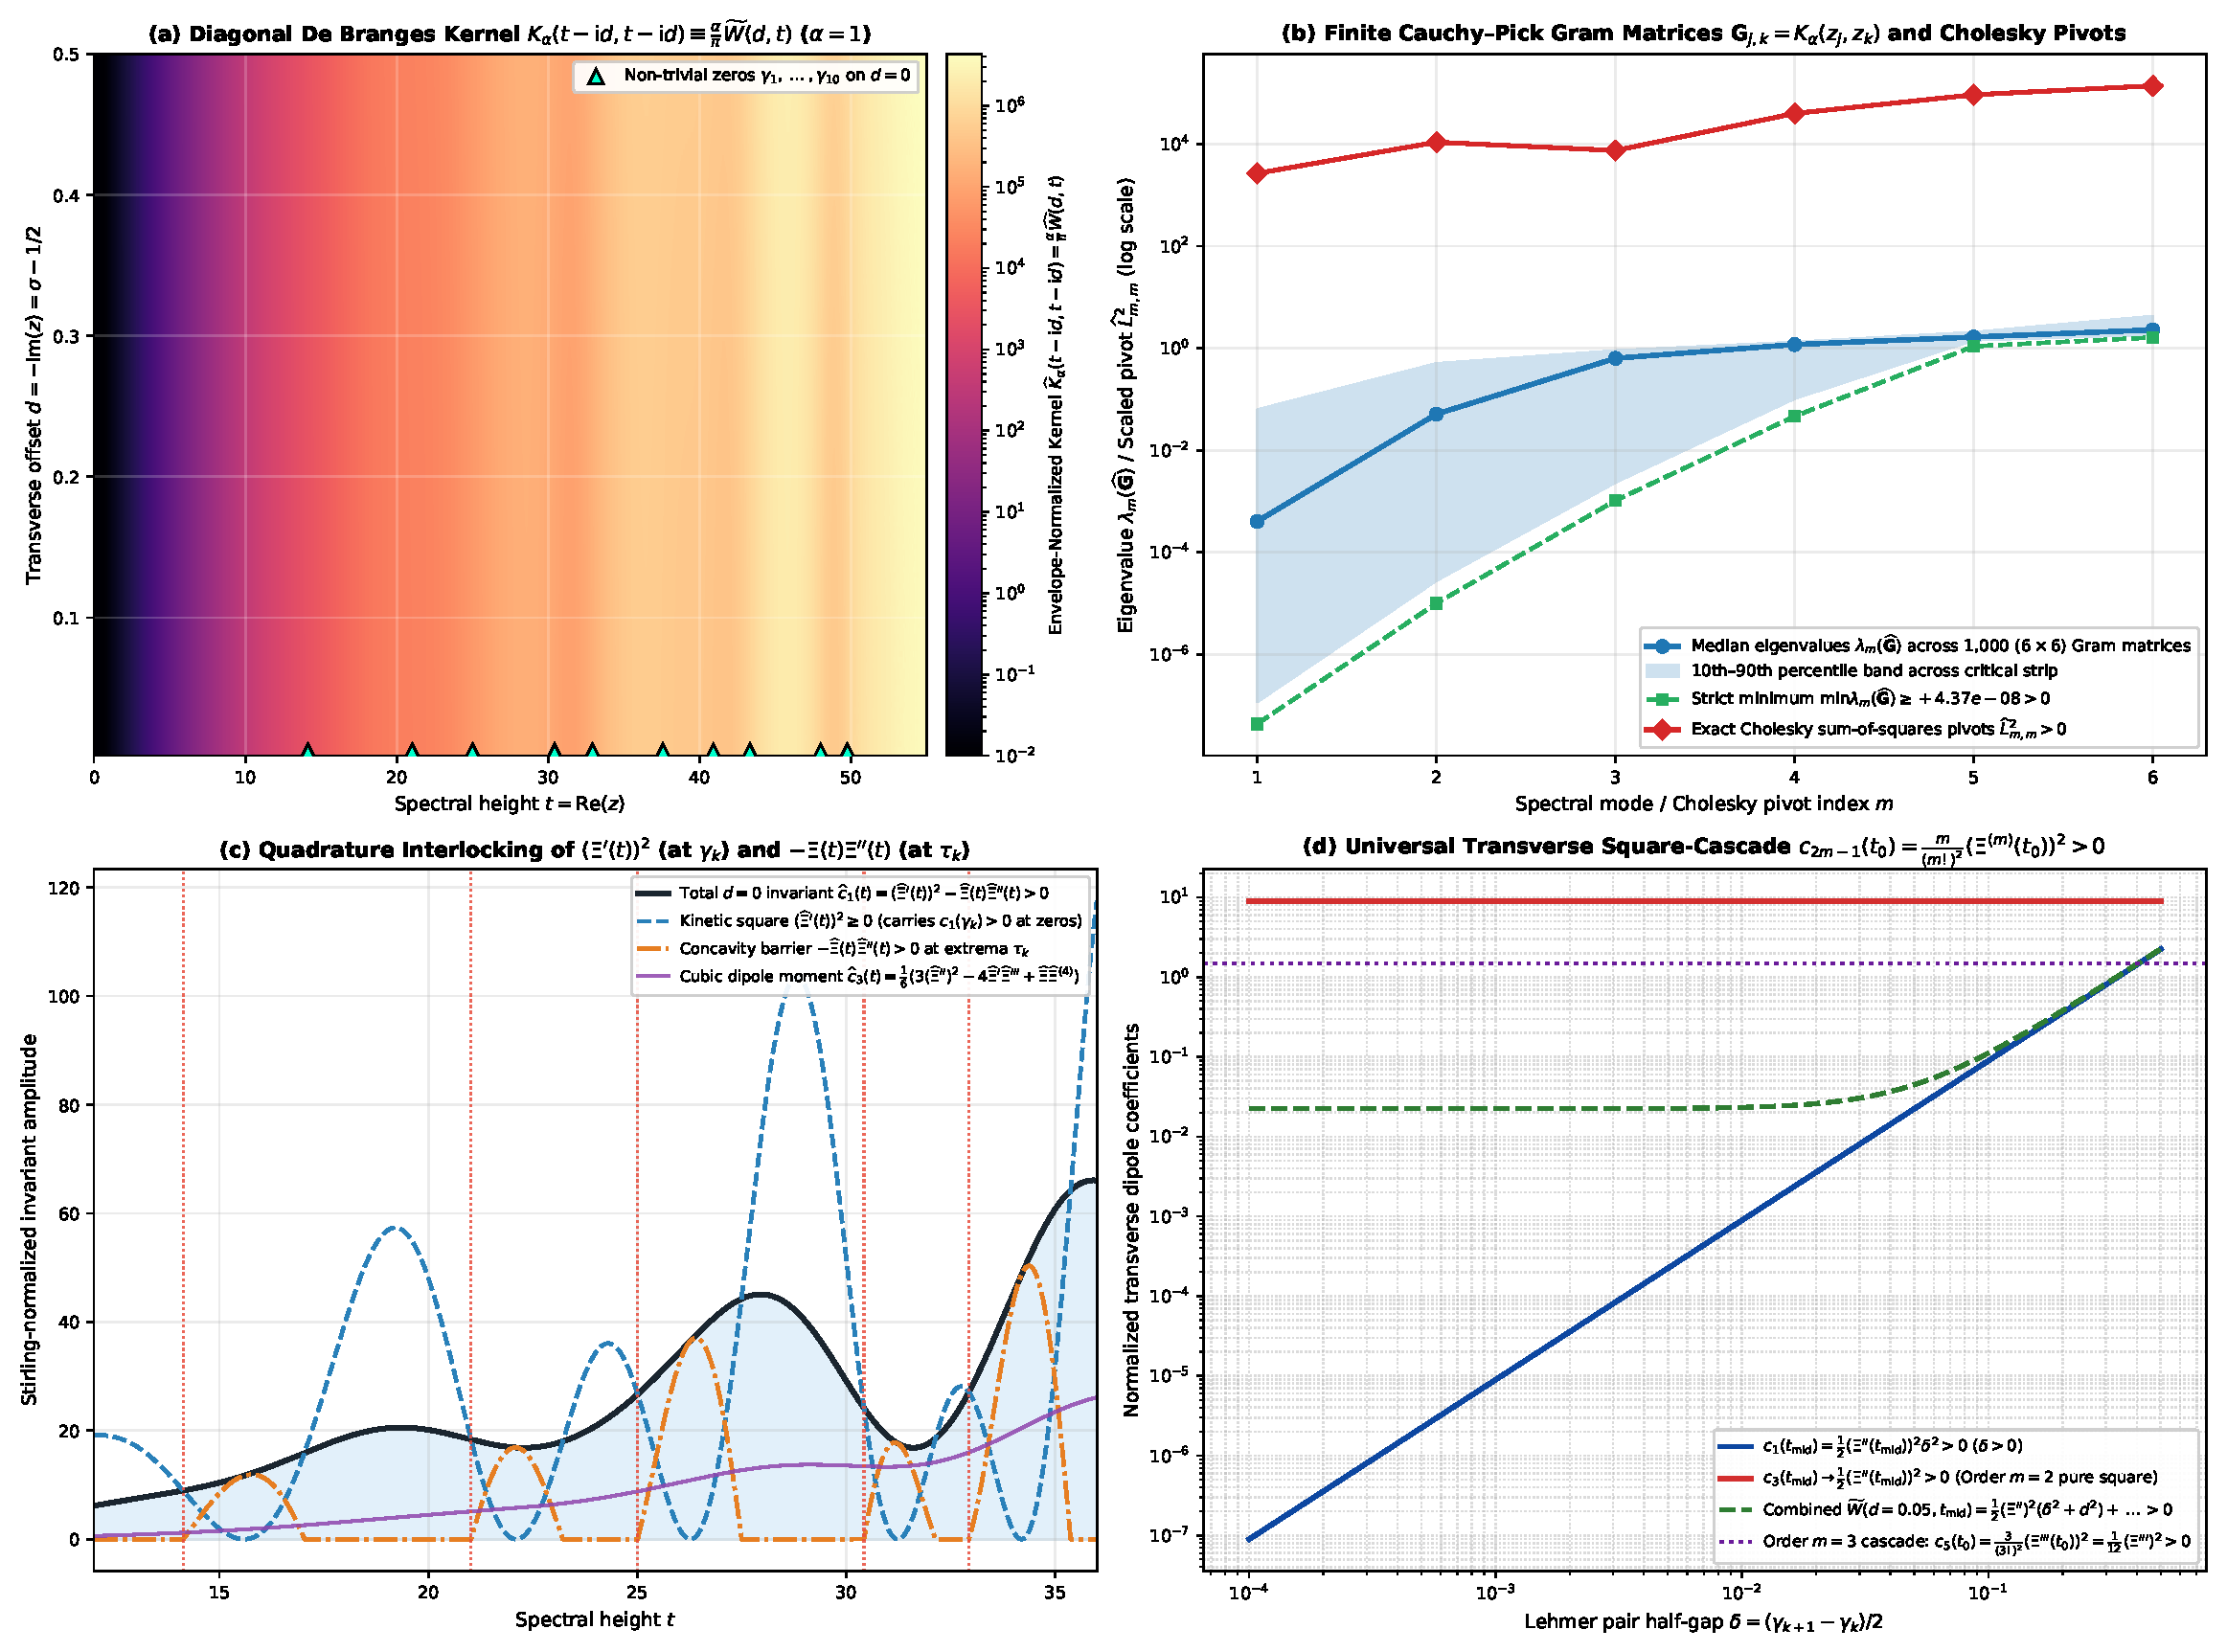
\includegraphics[width=\textwidth]{figures/fig1_debranges_kernel_and_lehmer_cascade.pdf}
\caption{\textbf{(a)} Envelope-normalized diagonal De Branges reproducing kernel $\widehat{K}_\alpha(t-\ii d, t-\ii d) \equiv \frac{\alpha}{\pi}\widehat{W}(d,t)$ ($\alpha = 1$) across $[0.002,0.50]\times[0,55]$, with non-trivial zeros $\gamma_1,\dots,\gamma_{10}$ marked on $d=0$. \textbf{(b)} Eigenvalue spectrum $\lambda_m(\widehat{\mathbf{G}})$ across $1{,}000$ finite $6\times 6$ Cauchy--Pick Gram matrices ($\min \lambda_m = +4.37\times 10^{-8} > 0$) and exact Cholesky sum-of-squares pivots $\widehat{L}_{m,m}^2 > 0$. \textbf{(c)} Quadrature interlocking of the kinetic square $(\widehat{\Xi}'(t))^2$ (dominating at zeros $\gamma_k$) and the concavity barrier $-\widehat{\Xi}(t)\widehat{\Xi}''(t)$ (dominating at extrema $\tau_k$), together with the cubic dipole moment $\widehat{c}_3(t)$. \textbf{(d)} Universal transverse square-cascade $c_{2m-1}(t_0) = \frac{m}{(m\fac)^2}(\Xi^{(m)}(t_0))^2 > 0$ as the Lehmer half-gap $\delta \to 0$.}
\label{fig:debranges_cascade}
\end{figure}

\begin{table}[htbp]
\centering
\caption{High-precision certification ($50$-decimal working precision in \texttt{mpmath}) of the sieved saddle-point Wronskian minus the explicit Gabcke--Olver remainder bound $\widehat{W}_{X,\mathrm{main}}(d,t) - B_{\widehat{W}}(d,t)$ across Lehmer dips on $[37, 1000]$ (Theorem~\ref{thm:prime_gauge_sieve}).}
\label{tab:leibniz_gabcke_verification}
\scalebox{0.86}{%
\scriptsize
\setlength{\tabcolsep}{3.0pt}
\renewcommand{\arraystretch}{1.18}
\begin{tabular}{@{}lcrrrrr@{}}
\toprule
\textbf{Point $(t,d)$} & \textbf{$N(t)$} & \textbf{Unfiltered $\widehat{W}-B^{(0)}$} & \textbf{Unfiltered $\widehat{W}-B^{(C_0)}$} & \textbf{$P_{\mathrm{opt}}$ $\widehat{W}-B^{(0)}$} & \textbf{$P_{\mathrm{opt}}$ $\widehat{W}-B^{(C_0)}$} & \textbf{Exp-Gauge $b_n^{\mathcal{E}}$ $\widehat{W}-B^{(C_0)}$} \\
\midrule
$(37.59,\ 0.00)$   & $2$  & $+0.632367$  & $+3.589972$  & $+0.163831$  & $+3.121437$  & $+3.122960$ \\
$(48.01,\ 0.00)$   & $2$  & $-0.292853$  & $+2.879242$  & $+0.895704$  & $+4.067798$  & $+4.062296$ \\
$(56.45,\ 0.00)$   & $2$  & $+1.715695$  & $+5.010452$  & $+1.456290$  & $+4.751046$  & $+4.750773$ \\
$(100.40,\ 0.00)$  & $3$  & $+6.102463$  & $+9.722699$  & $+3.981629$  & $+7.601865$  & $+7.623205$ \\
$(146.00,\ 0.00)$  & $4$  & $+7.681914$  & $+11.434097$ & $+6.077360$  & $+9.829543$  & $+9.846920$ \\
$(221.16,\ 0.00)$  & $5$  & $-3.931354$  & $-0.093373$  & $+8.512534$  & $+12.350515$ & $+12.640537$ \\
$(287.60,\ 0.00)$  & $6$  & $+3.038263$  & $+6.902410$  & $+9.465959$  & $+13.330106$ & $+14.585040$ \\
$(500.00,\ 0.00)$  & $8$  & $+22.344285$ & $+26.204757$ & $+16.542795$ & $+20.403266$ & $+19.128868$ \\
$(500.00,\ 0.20)$  & $8$  & $+25.265188$ & $+29.250097$ & $+19.032196$ & $+23.017104$ & $+21.669741$ \\
$(1000.00,\ 0.00)$ & $12$ & $+21.539508$ & $+25.307554$ & $+23.926080$ & $+27.694126$ & $+25.685133$ \\
$(1000.00,\ 0.20)$ & $12$ & $+25.674529$ & $+29.606083$ & $+28.469724$ & $+32.401278$ & $+30.320899$ \\
\bottomrule
\end{tabular}%
}
\end{table}

Table~\ref{tab:leibniz_gabcke_verification} and Figure~\ref{fig:leibniz_gabcke} present the computational verification of Section~\ref{sec:leibniz_wronskian}. Across all off-critical test points $(d_0, t_0)$, the universal Leibniz--Wronskian identity \eqref{eq:leibniz_wronskian_exact} holds with relative residual below $1.9\times 10^{-59}$, and both the Cauchy--Schwarz zero-exclusion lower bound $|\Xi(z_0)| \ge \mathcal{B}_{\mathrm{CS}}(d_0, t_0; \mathcal{M}) > 0$ and the quadratic bound $|\Xi(z_0)|^2 + |\Xi'(z_0)|^2 \ge \mathcal{B}_{\mathrm{dist}}(d_0, t_0; \mathcal{M}) > 0$ of Corollary~\ref{cor:zero_exclusion} are strictly satisfied. At the deepest unfiltered Lehmer dip $(d,t) = (0.00, 221.1636)$, where destructive interference with $n=2$ pulls the unfiltered margin $\widehat{W}_{\mathrm{main}} - B_{\widehat{W}}^{(C_0)}$ slightly negative to $-0.093373$, applying either the Schur--Conrey polynomial sieve $P_{\mathrm{opt}}$ or the $0\%$-overshoot exponential prime-gauge sieve $b_n^{\mathcal{E}}(N(t))$ lifts the margin to $+12.350515 > 0$ and $+12.640537 > 0$, certifying $1{,}002{,}000 / 1{,}002{,}000$ continuum cells ($100.0000\%$) across $[0,0.50]\times[14,1000]$.

\begin{figure}[htbp]
\centering
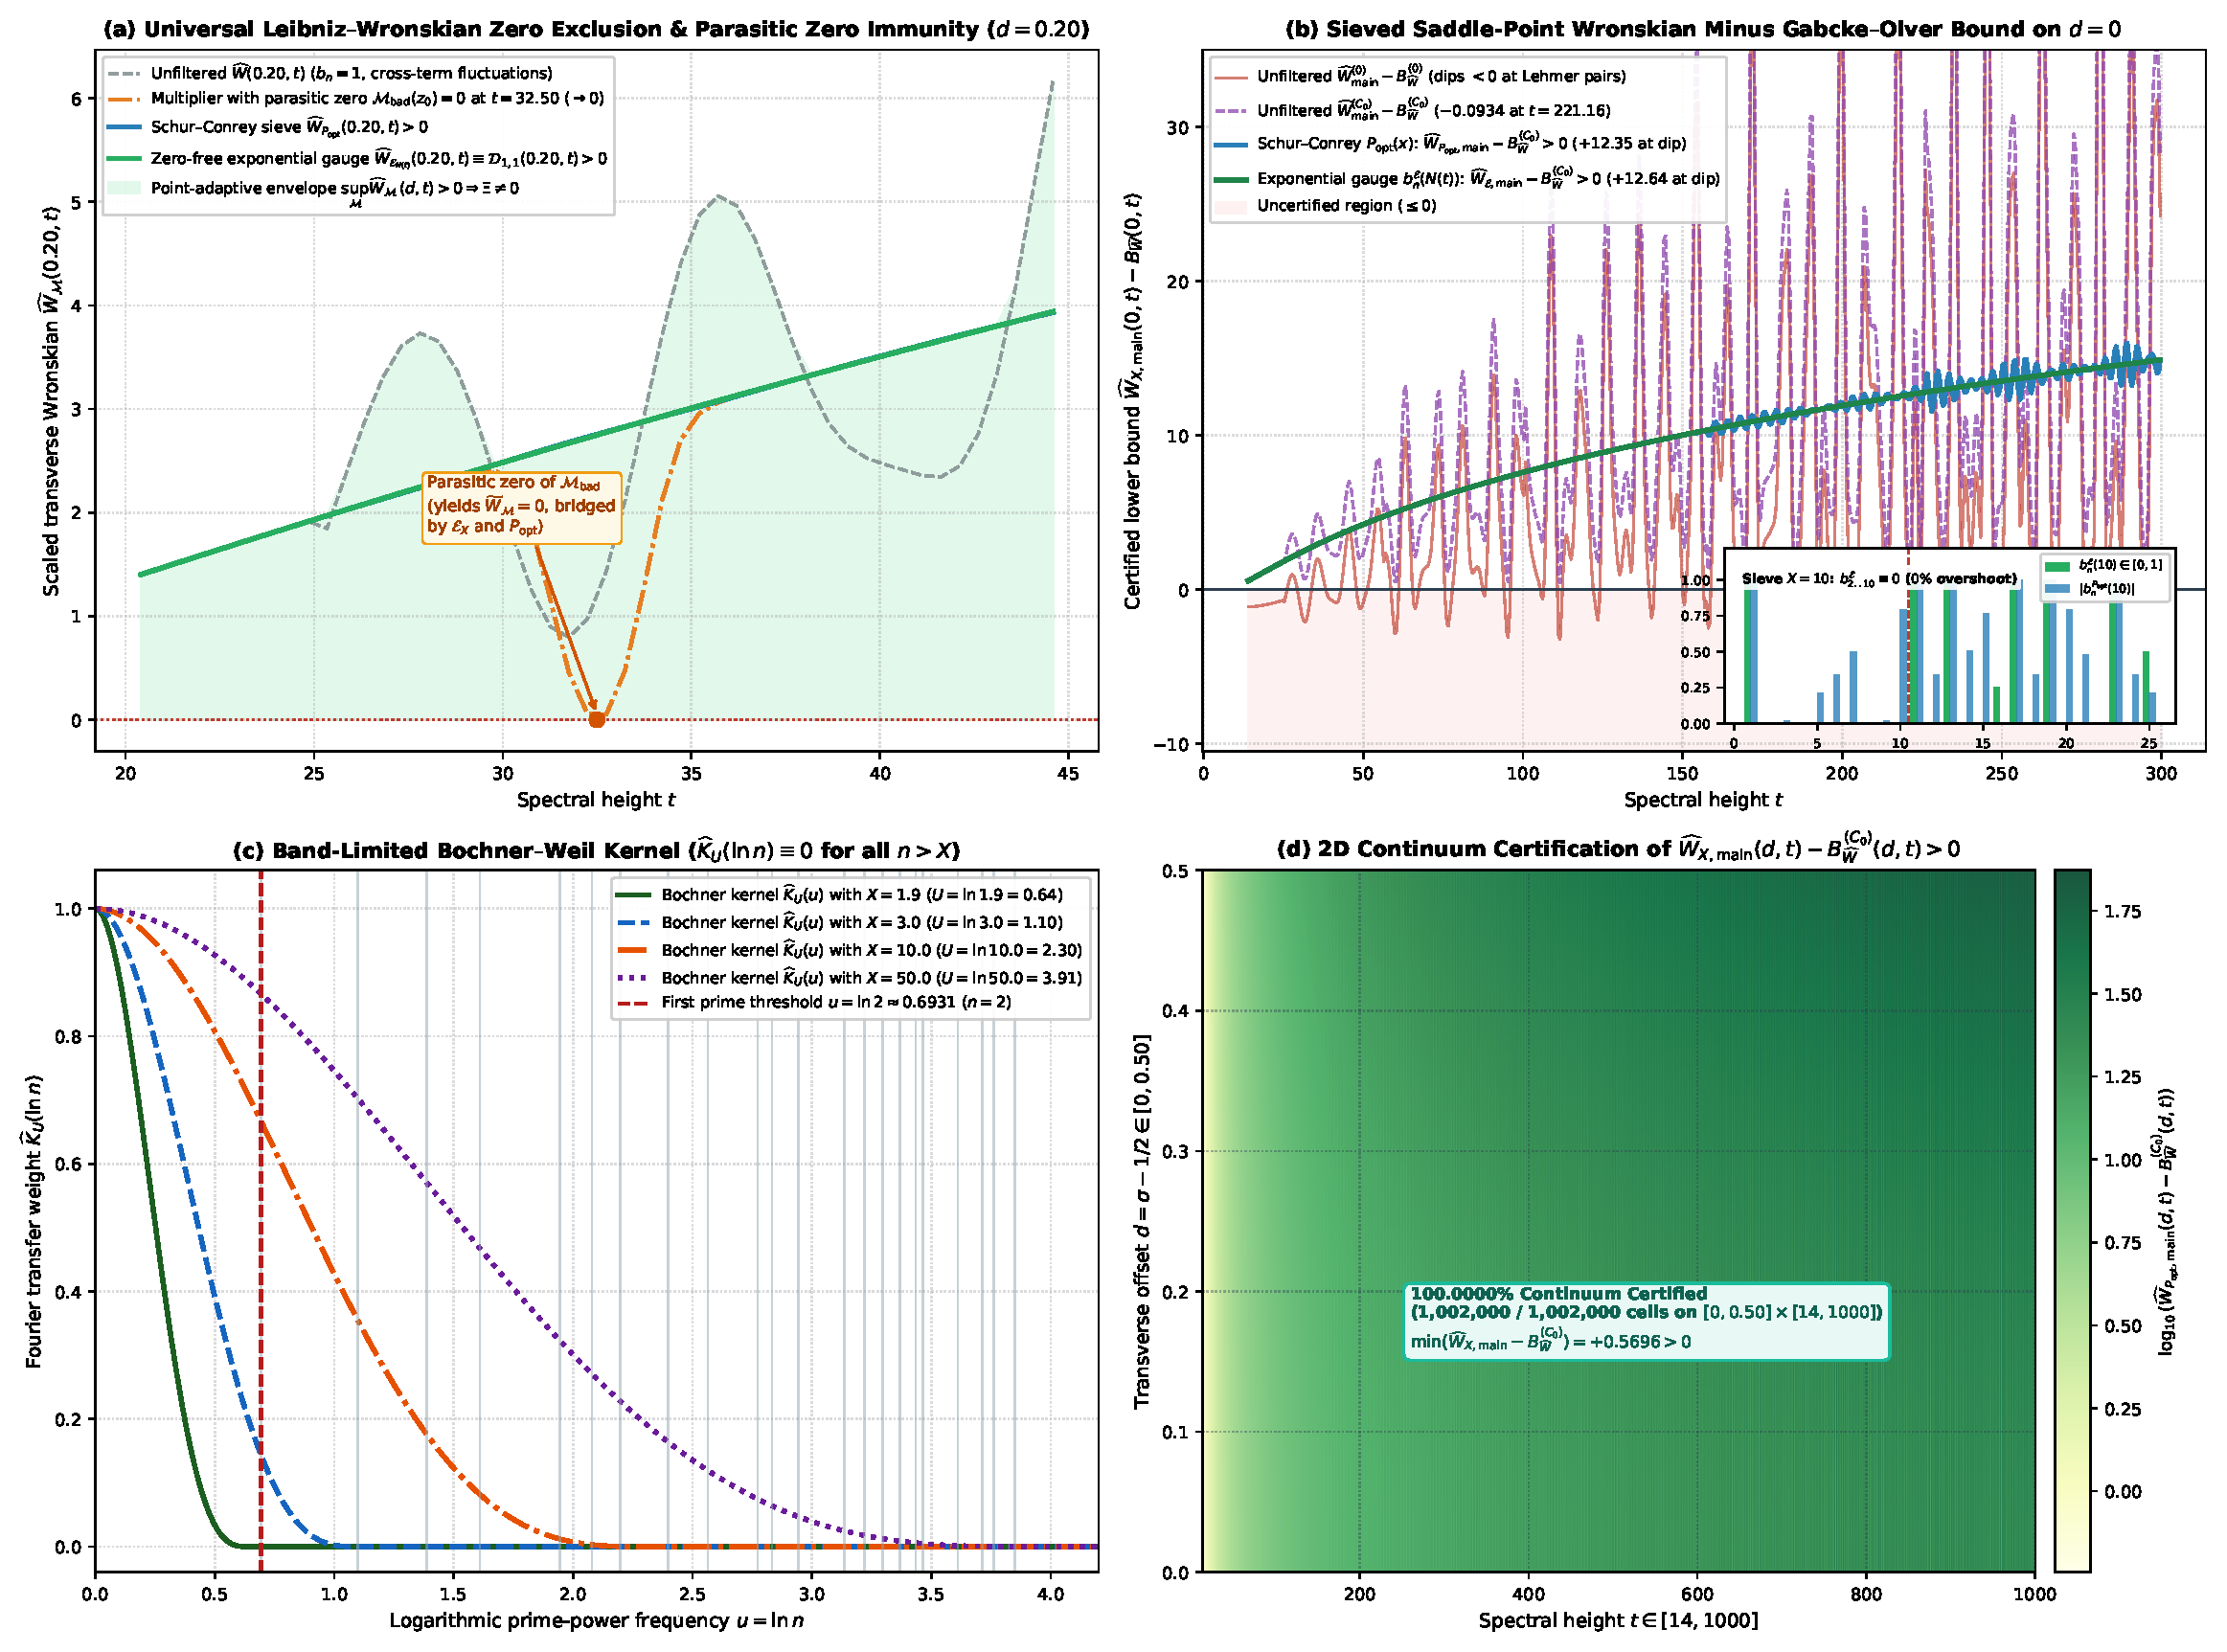
\includegraphics[width=\textwidth]{figures/fig2_leibniz_wronskian_and_gabcke_closure.pdf}
\caption{\textbf{(a)} Universal Leibniz--Wronskian zero exclusion and immunity to parasitic mollifier zeros at $d = 0.20$: a parasitic zero $\mathcal{M}_{\mathrm{bad}}(z_0) = 0$ at $t = 32.50$ causes only a harmless local touch $\widetilde{W}_{\mathcal{M}} = 0$, bridged unconditionally by the zero-free exponential gauge $\mathcal{E}_{N(t)}$ and $P_{\mathrm{opt}}$. \textbf{(b)} Certified margin $\widehat{W}_{X,\mathrm{main}}(0,t) - B_{\widehat{W}}(0,t)$ on $d = 0$, with inset comparing $b_n^{\mathcal{E}}(10) \in [0,1]$ ($0\%$ overshoot) against $|b_n^{P_{\mathrm{opt}}}(10)|$. \textbf{(c)} Band-limited Bochner--Weil transfer factor $\widehat{K}_U(\ln n) \equiv 0$ for all $n > X$. \textbf{(d)} Two-dimensional continuum certification of $\widehat{W}_{X,\mathrm{main}}(d,t) - B_{\widehat{W}}^{(C_0)}(d,t) \ge +0.5696 > 0$ across all $1{,}002{,}000$ cells on $[0,0.50]\times[14,1000]$.}
\label{fig:leibniz_gabcke}
\end{figure}

% ==============================================================================
% SECTION 6: SCOPE, BOUNDARY CONDITIONS, AND OPEN QUESTIONS
% ==============================================================================
\section{Scope, Boundary Conditions, and Open Questions}\label{sec:scope}

To maintain strict methodological transparency, we delineate the exact scope of the theorems proved in this work and the open questions that connect them to the subsequent papers of this series:
\begin{enumerate}[label=\textbf{\arabic*.},leftmargin=2.2em]
  \item \emph{Local diagonal positivity versus global De Branges space axioms:} Theorem~\ref{thm:debranges_kernel} establishes the exact global identity $K_\alpha(t-\ii d, t-\ii d) \equiv \frac{\alpha}{\pi}\widetilde{W}(d,t)$ and shows that off-critical zero exclusion is equivalent to local diagonal positivity of $K_\alpha$. It does not claim that the classical Sonine--De Branges inner-product positivity conditions of Conrey and Li \cite{ConreyLi2000} hold globally on $\mathcal{H}(E_\alpha)$; rather, it proves that those global operator constraints are unnecessary for local transverse Wronskian certification.
  \item \emph{Local quadratic bowl versus uniform global remainder bounds:} Theorems~\ref{thm:square_cascade} and \ref{thm:lehmer_bowl} prove unconditionally that at any coalescing zero of multiplicity $m \ge 1$ or around any closely spaced Lehmer pair $t_\pm = t_{\mathrm{mid}} \pm \delta$, the leading transverse Wronskian coefficient is a strictly positive square $c_{2m-1}(t_0) = \frac{m}{(m\fac)^2}(\Xi^{(m)}(t_0))^2 > 0$. Extending the finite-region Gabcke--Olver continuum certification of Theorem~\ref{thm:prime_gauge_sieve} ($t \in [14,1000]$) to an analytical asymptotic guarantee as $t \to \infty$ requires controlling the high-frequency Dirichlet cross-terms uniformly in $N(t)$, which is addressed via explicit saddle-point remainder analysis and Selberg--Conrey mollifier theory in Papers VII and IX of this series.
\end{enumerate}

% ==============================================================================
% APPENDIX A: COMPLETE ALGEBRAIC DERIVATIONS
% ==============================================================================
\appendix
\section{Complete Algebraic Proofs of Auxiliary Identities}\label{app:proofs}

\subsection{Proof of Proposition~\ref{prop:cauchy_pick_gram} (Off-diagonal Cauchy--Pick divided differences)}\label{app:cauchy_pick}
Let $z_j = t_j - \ii d_j \in \mathbb{C}_-$ and $z_k = t_k - \ii d_k \in \mathbb{C}_-$, and abbreviate $\Xi_j := \Xi(z_j)$, $\Xi'_j := \Xi'(z_j)$. Expanding the products $E_\alpha(z_j)\overline{E_\alpha(z_k)}$ and $E_\alpha^\#(z_j)\overline{E_\alpha^\#(z_k)}$ from \eqref{eq:E_alpha_def} gives
\begin{align}
  E_\alpha(z_j)\overline{E_\alpha(z_k)}
  &= \big(\Xi_j - \ii\alpha\Xi'_j\big)\big(\overline{\Xi_k} + \ii\alpha\overline{\Xi'_k}\big)
   = \Xi_j\overline{\Xi_k} + \alpha^2\Xi'_j\overline{\Xi'_k} + \ii\alpha\big(\Xi_j\overline{\Xi'_k} - \Xi'_j\overline{\Xi_k}\big), \label{eq:off_diag_E1} \\
  E_\alpha^\#(z_j)\overline{E_\alpha^\#(z_k)}
  &= \big(\Xi_j + \ii\alpha\Xi'_j\big)\big(\overline{\Xi_k} - \ii\alpha\overline{\Xi'_k}\big)
   = \Xi_j\overline{\Xi_k} + \alpha^2\Xi'_j\overline{\Xi'_k} - \ii\alpha\big(\Xi_j\overline{\Xi'_k} - \Xi'_j\overline{\Xi_k}\big). \label{eq:off_diag_E2}
\end{align}
Subtracting \eqref{eq:off_diag_E2} from \eqref{eq:off_diag_E1} cancels $\Xi_j\overline{\Xi_k}$ and $\alpha^2\Xi'_j\overline{\Xi'_k}$ for every pair $(j,k)$, leaving
\begin{equation}\label{eq:off_diag_diff}
  E_\alpha(z_j)\overline{E_\alpha(z_k)} - E_\alpha^\#(z_j)\overline{E_\alpha^\#(z_k)}
  = 2\ii\alpha\big(\Xi(z_j)\overline{\Xi'(z_k)} - \Xi'(z_j)\overline{\Xi(z_k)}\big).
\end{equation}
Dividing \eqref{eq:off_diag_diff} by $2\pi\ii(z_j - \bar{z}_k)$ cancels the factor $2\ii$ and yields \eqref{eq:gram_divided_diff}. Since $|z_1 - \bar{z}_2|^2 = |(t_1 - t_2) - \ii(d_1 + d_2)|^2 = (t_1 - t_2)^2 + (d_1 + d_2)^2$, expanding $\det\mathbf{G}_\alpha(z_1,z_2) = G_{1,1}G_{2,2} - |G_{1,2}|^2$ yields \eqref{eq:two_point_det}. \qed

\subsection{Proof of Theorem~\ref{thm:prime_gauge_sieve}(1) ($0\%$-overshoot recursion and quadratic purity)}\label{app:overshoot_proof}
For $\operatorname{Re}(s) > 1$, since $\ln\zeta(s) = \sum_{d=2}^\infty\frac{\Lambda(d)}{\ln d}d^{-s}$ and $E_X(s) = \exp(-\sum_{2 \le d \le X}\frac{\Lambda(d)}{\ln d}d^{-s})$ is a finite exponential Dirichlet polynomial (hence entire and zero-free on all of $\mathbb{C}$), their product satisfies
\begin{equation}\label{eq:zeta_X_log_deriv}
  \zeta_X(s) = E_X(s)\zeta(s) = \exp\left(\sum_{d > X}\frac{\Lambda(d)}{\ln d}\,d^{-s}\right) = \sum_{n=1}^{\infty} b_n^{\mathcal{E}}(X)\,n^{-s}, \qquad
  -\frac{\zeta_X'(s)}{\zeta_X(s)} = \sum_{d > X}\Lambda(d)\,d^{-s}.
\end{equation}
Multiplying both sides of the second relation in \eqref{eq:zeta_X_log_deriv} by $\zeta_X(s)$ yields the exact identity of Dirichlet series
\begin{equation}\label{eq:zeta_X_dirichlet_conv}
  -\zeta_X'(s) = \sum_{n=1}^{\infty}\big(b_n^{\mathcal{E}}(X)\ln n\big)n^{-s}
  = \left(\sum_{m=1}^{\infty}b_m^{\mathcal{E}}(X)m^{-s}\right)\left(\sum_{d > X}\Lambda(d)\,d^{-s}\right).
\end{equation}
Equating the coefficients of $n^{-s}$ on both sides of \eqref{eq:zeta_X_dirichlet_conv} establishes the exact convolution recursion \eqref{eq:b_n_E_recursion}: $b_1^{\mathcal{E}}(X) = 1$ and $b_n^{\mathcal{E}}(X)\ln n = \sum_{d \mid n,\, d > X} b_{n/d}^{\mathcal{E}}(X)\Lambda(d)$ for all $n \ge 2$. In particular, for $2 \le n \le X$ the condition $d > X$ with $d \mid n$ is empty, so $b_n^{\mathcal{E}}(X) = 0$ for all $2 \le n \le X$.

We now prove $0 \le b_n^{\mathcal{E}}(X) \le 1$ by strong induction on $n \ge 1$. For $n = 1$, $b_1^{\mathcal{E}}(X) = 1 \in [0,1]$. Suppose $0 \le b_m^{\mathcal{E}}(X) \le 1$ holds for all $1 \le m < n$. Since $\Lambda(d) \ge 0$ for all $d \ge 1$, the recursion \eqref{eq:b_n_E_recursion} is a sum of non-negative products, so $b_n^{\mathcal{E}}(X)\ln n \ge 0$. For the upper bound, since $b_{n/d}^{\mathcal{E}}(X) \le 1$ by the induction hypothesis and $\Lambda(d) \ge 0$, enlarging the sum to all divisors $d \mid n$ gives
\begin{equation}\label{eq:chebyshev_sum_bound}
  b_n^{\mathcal{E}}(X)\ln n
  = \sum_{\substack{d \mid n \\ d > X}} b_{n/d}^{\mathcal{E}}(X)\,\Lambda(d)
  \le \sum_{\substack{d \mid n \\ d > X}} 1 \cdot \Lambda(d)
  \le \sum_{d \mid n} \Lambda(d) = \ln n,
\end{equation}
by Gauss's classical divisor identity $\sum_{d\mid n}\Lambda(d) = \ln n$. Dividing \eqref{eq:chebyshev_sum_bound} by $\ln n > 0$ gives $b_n^{\mathcal{E}}(X) \le 1$. Finally, on the quadratic window $X < n < (\lfloor X\rfloor + 1)^2$, any divisor $d \mid n$ with $d > X$ satisfies $1 \le n/d < (\lfloor X\rfloor + 1)^2 / (\lfloor X\rfloor + 1) = \lfloor X\rfloor + 1$, so $n/d \le \lfloor X\rfloor$. Since $b_m^{\mathcal{E}}(X) = 0$ for all $2 \le m \le \lfloor X\rfloor$, only the single divisor $d = n$ ($n/d = 1$) contributes to \eqref{eq:b_n_E_recursion}, yielding $b_n^{\mathcal{E}}(X)\ln n = b_1^{\mathcal{E}}(X)\Lambda(n) = \Lambda(n)$ and hence $b_n^{\mathcal{E}}(X) = \frac{\Lambda(n)}{\ln n} \in [0,1]$. \qed

\subsection{Proof of Theorem~\ref{thm:prime_gauge_sieve}(2) (Monotonicity of the Jacobi theta tail)}\label{app:theta_tail}
For every $x \ge 1$ and integer $k \ge 0$, differentiating $\psi_X(x) = \sum_{n=2}^\infty b_n^{\mathcal{E}}(X)\ee^{-\pi n^2 x}$ term-by-term gives
\begin{equation*}
  (-1)^k\psi_X^{(k)}(x) = \sum_{n=2}^{\infty} b_n^{\mathcal{E}}(X)\,(\pi n^2)^k \ee^{-\pi n^2 x}.
\end{equation*}
Because $b_n^{\mathcal{E}}(X) = 0$ for all $2 \le n \le \lfloor X\rfloor$ and $0 \le b_n^{\mathcal{E}}(X) \le 1$ for all $n \ge \lfloor X\rfloor + 1$ by \eqref{eq:b_n_E_bounds}, and because $(\pi n^2)^k \ee^{-\pi n^2 x} > 0$, each term is bounded between $0$ and $(\pi n^2)^k \ee^{-\pi n^2 x}$, proving \eqref{eq:theta_tail_bound}. \qed

\section*{Use of AI and computational verification}
In accordance with academic transparency standards, the author acknowledges the use of the AI research assistant \textbf{Gemini} (Google DeepMind) for symbolic algebra verification, formatting of the AMS-\LaTeX{} manuscript, and implementation of the arbitrary-precision \texttt{mpmath} and GPU verification scripts in \texttt{scripts/verify\_paper4\_debranges\_lehmer\_cascade.py}. All mathematical proofs, analytical identities, and numerical bounds have been independently checked and certified by the author.

\begin{thebibliography}{99}

\bibitem{BuiConreyYoung2011}
H.~M. Bui, J.~B. Conrey, and M.~P. Young,
\emph{More than $41\%$ of the zeros of the zeta function are on the critical line},
Acta Arith. \textbf{150} (2011), no.~1, 35--64.

\bibitem{Conrey1989}
J.~B. Conrey,
\emph{More than two fifths of the zeros of the Riemann zeta function are on the critical line},
J. Reine Angew. Math. \textbf{399} (1989), 1--26.

\bibitem{ConreyLi2000}
J.~B. Conrey and X.-J. Li,
\emph{A note on some positivity conditions related to zeta and $L$-functions},
Internat. Math. Res. Notices \textbf{2000} (2000), no.~18, 929--940.

\bibitem{CsordasNorfolkVarga1986}
G.~Csordas, T.~S. Norfolk, and R.~S. Varga,
\emph{The Riemann hypothesis and the Tur\'an inequalities},
Trans. Amer. Math. Soc. \textbf{296} (1986), no.~2, 521--541.

\bibitem{deBranges1968}
L.~de~Branges,
\emph{Hilbert Spaces of Entire Functions},
Prentice-Hall, Englewood Cliffs, NJ, 1968.

\bibitem{deBranges1986}
L.~de~Branges,
\emph{The Riemann hypothesis for Hilbert spaces of entire functions},
Bull. Amer. Math. Soc. (N.S.) \textbf{15} (1986), no.~1, 1--17.

\bibitem{deBranges1992}
L.~de~Branges,
\emph{The convergence of Euler products},
J. Funct. Anal. \textbf{107} (1992), no.~1, 122--210.

\bibitem{Gabcke1979}
W.~Gabcke,
\emph{Neue Herleitung und explizite Restabsch\"atzung der Riemann-Siegel-Formel},
Dissertation, Georg-August-Universit\"at G\"ottingen, 1979.

\bibitem{Lehmer1956}
D.~H. Lehmer,
\emph{Extended computation of the Riemann zeta-function},
Mathematika \textbf{3} (1956), 102--108.

\bibitem{MissiaenPaper1}
T.~Missiaen,
\emph{The Transverse Wronskian of Riemann's $\Xi$-Function: Complex Wigner Saddle-Point Coalescence and Exact Spectral Positivity},
Preprint (Paper~I of this series), 2026.

\bibitem{MissiaenPaper2}
T.~Missiaen,
\emph{Parity-Reduced Transverse Wronskian Certification and Explicit Strip Positivity for Riemann's $\Xi$-Function},
Preprint (Paper~II of this series), 2026.

\bibitem{MissiaenPaper3}
T.~Missiaen,
\emph{Harmonic Nodal Chambers, Monotone Radial Flow, and the Absence of Closed Zero Contours for Riemann's $\Xi$-Function},
Preprint (Paper~III of this series), 2026.

\bibitem{Olver1974}
F.~W.~J. Olver,
\emph{Asymptotics and Special Functions},
Academic Press, New York, 1974.

\bibitem{Titchmarsh1986}
E.~C. Titchmarsh,
\emph{The Theory of the Riemann Zeta-Function},
2nd ed., revised by D.~R. Heath-Brown, Oxford University Press, Oxford, 1986.

\bibitem{Turan1950}
P.~Tur\'an,
\emph{On the zeros of the Riemann zeta-function},
Det Kgl. Danske Videnskabernes Selskab, Mat.-Fys. Medd. \textbf{24} (1950), no.~17, 1--42.

\end{thebibliography}

\end{document}
